\chapter{Implementation} \label{ch:implementation}
The \textit{Hyper} video game is a relatively big project (it comprises around 260 classes), so naturally we have to contain the discussion to only the most important parts of the system.
Conceptually, there are four different "areas" spanned by the project:
\begin{enumerate}
  \item game objects management,
  \item procedural world generation,
  \item rendering,
  \item user interface.
\end{enumerate}

In what follows, we will discuss these areas in more detail.
We will also provide information on the technologies used in the project and present its core components.

\section{Technologies selection}\label{sec:technologies_selection}
The video game is written in C\# and uses OpenGL Shading Language (GLSL) for the shaders.
The targeted platform is .NET 7 on Windows 10 and above.

The game relies on the following third-party libraries:
\begin{itemize}
    \item OpenTK\footnote{\url{https://github.com/opentk/opentk}} -- a set of low-level C\# bindings for OpenGL; used for 3D rendering,
    \item BepuPhysics2\footnote{\url{https://github.com/bepu/bepuphysics2}} -- a low-level, highly performant physics simulation library; used as the physics engine,
    \item SkiaSharp\footnote{\url{https://github.com/mono/SkiaSharp}} -- API for rendering 2D images; used for 2D rendering (menus, controls, etc.),
    \item AssimpNet\footnote{\url{https://github.com/MonoGame/AssimpNet}} -- a .NET wrapper for the Open Asset Import (Assimp) library\footnote{\url{https://assimp.org/}}; used for loading models,
    \item StbImageSharp\footnote{\url{https://github.com/StbSharp/StbImageSharp}} -- C\# port of the \texttt{stb\_image.h} header file; used for loading images.
\end{itemize}
\section{Game objects management}
A game object, such as a humanoid-looking bot or a car most often can be understood as existing in three different planes simultaneously:
\begin{enumerate}
    \item the visual layer,
    \item the physical layer,
    \item the logical layer.
\end{enumerate}
The visual layer of an object describes how the object looks like during the gameplay.
This side of a game object we will call a \textit{model}.
The information about models (vertices, normal vectors, UV mappings, textures, and animations) is read from COLLADA and PNG files (cf. \autoref{subsec:model_loader-class}) and stored in the \texttt{Model} class.
It's important to note that if multiple game objects look the same, the model information is shared between them in the form of a single \texttt{ModelResource} class instance.
More specifically, the \texttt{ModelResource} class is abstract, and its derived classes are singletons.
Animated models additionally use the \texttt{Aminator} class (cf. \autoref{subsec:animator-class}) which provides a way to calculate the bone transforms based on the elapsed time.
Some models are \textit{compound}.
The car model, for example, stores information about the look of the wheels and body separately.

The physical layer defines the physical properties of the game object at any given moment.
Some basic ones include inertia, angular and linear velocity, and friction;
in the case of more complex objects such as a car, the description contains information about \textit{constraints}.
The constraints define the relative positions of different elements of the object and their velocities.
An example of a constraint would be the wheel axes of the car.
It's worth noting that the position constraints don't have to be "stiff" (they are modeled as springs).
Technically, once a game object is added to the simulation, it is represented by one (or more in the case of compound bodies) \textit{body handle}.
Therefore, each game object has to implement the \texttt{ISimulationMember} interface which has a property that returns the list of all body handles associated with the given game object.
More details on coupling the physics engine with the rest of the game can be found in \autoref{subsec:physics-project}

The logical layer is the soul of each object.
NPCs move in a way given by a simple algorithm;
the player can inflict damage to NPCs by shooting projectiles, and so on.
Game objects can react to collisions with other objects by registering for contact callbacks, i.e. implementing the \texttt{IContactEventListener} interface.
They can also move (either on their own, like NPCs, or due to the player input) by registering input callbacks, i.e. implementing the \texttt{IInputSubscriber} interface (cf. \autoref{subsec:context-class} and \autoref{subsec:transporter-classes}).
The logic related to game objects of a given kind is usually contained in a respective Controller class, described in more detail in \autoref{subsec:controller-classes}.

All game objects are members of a scene (cf. \autoref{subsec:scene-class}).

In the remainder of this section, we will cover some of the most important components related to managing game objects.
\subsection{\texttt{Animator} class}\label{subsec:animator-class}

The \texttt{Animator} class is responsible for animating the models loaded by \texttt{ModelLoader}.
It takes animation keyframes and interpolates them using Quaternion Slerp and Vector3 Lerp which are provided by AssimpNet.
It then uses the interpolated keyframes to calculate the transformation matrices for each bone in the model which are later passed to the shader.
The logic is described in more detail in \autoref{sec:theory_theory_models}.
\subsection{\texttt{ModelLoader} class}\label{subsec:model_loader-class}

The model loader is responsible for loading models from the file system.
It loads COLLADA files using AssipmNet to convert them to model class objects.
Each vertex in the mesh of the model must be dependent on at most 4 bones.
It creates VAOs for each mesh of the model, stores them in the Model class object, loads a PNG file, and stores it in a Texture class object.

\subsection{\texttt{Physics} project}\label{subsec:physics-project}
The Physics component is responsible for collision detection, ray casting, and physical modeling.
The main purpose of this component is to expose the various functionalities of the BepuPhysics2 library to the rest of the system.
The component also makes extensive use of the code from the BepuPhysics2 Demos project.

Each game object is represented by a \textit{body} (each body has an associated \textit{body handle}) in the physics engine.
This one-to-one mapping is stored in the \texttt{Scene} class in an object of \texttt{SimulationMembers} type.
\texttt{SimulationMembers} allows for adding and removing simulation members as well as accessing handles to bodies in the physics engine associated with a given game object.
Game objects are represented by either simple or composite shapes in the physical simulation.
Simple shapes used in the game include cylinders, capsules, and boxes.
Composite shapes arise by composing simple shapes.

To facilitate debugging, the Physics component also provides a way to extract all shapes from the simulation (and decompose composite shapes) which then can be shown in debug mode, see \autoref{fig:bounding-shapes}.
When shown, the bounding shapes can be either green or red depending on whether the corresponding bodies are in the active or inactive state in the physics engine.
In \autoref{fig:bounding-shapes} it can be seen that the player has been hit by a projectile which caused the player's body to become active (or \textit{awakend} using the BepuPhysics parlance) as indicated by the green bounding shape.
The projectile that hit the player can also be seen to be active.
On the other hand, the projectiles that fell to the ground and had been still for some time became inactive as marked by the red bounding shapes.
\begin{figure}[h]
    \centering
    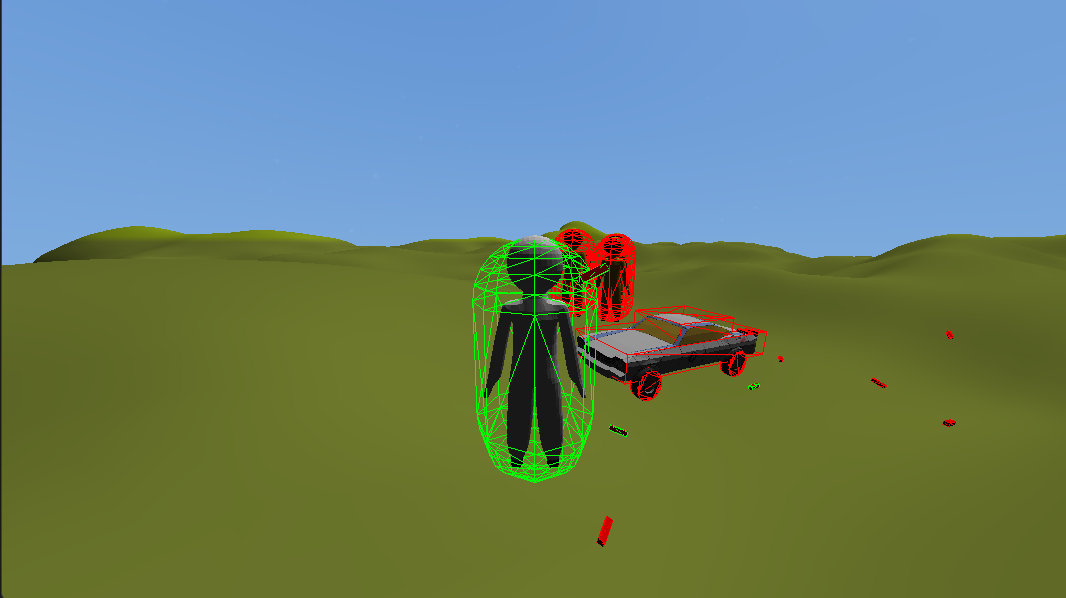
\includegraphics[width=0.8\textwidth]{chapters/implementation/sections/game_objects_management/subsections/physics_project/resources/bounding-shapes.png}
    \caption{Game objects enclosed in bounding shapes for collision detection}
    \label{fig:bounding-shapes}
\end{figure}

The body that represents the terrain was created as a separate shape from the terrain mesh triangle-by-triangle.

Game objects can listen and respond to collisions by registering their contact callbacks via the API in \texttt{SimulationManager}.
Such objects implement the \texttt{IContactEventListener} interface whose implementations define the contact callbacks.
The only information about the collision is which two bodies collided and where.

Some game objects can cast rays.
An example of such an object is the player who uses a ray to define a place where terrain modification should take place.
Each ray in the physics engine has an ID number, direction, etc.
An object that wishes to cast rays has to therefore implement an interface (\texttt{IRayCaster}) that exposes all the necessary information.
\subsection{\texttt{Scene} class} \label{subsec:scene-class}
The \texttt{Scene} class is responsible for storing all the objects in the game the player can interact with.
It is also responsible for releasing the objects' resources.
Some of the objects stored in the \texttt{Scene}'s instance are the following: car, chunks, player, camera, etc.
\subsection{\texttt{*Controller} classes}
There are eight controller classes in the project:
\texttt{PlayerController},
\texttt{BotsController},
\texttt{ChunksController},
\texttt{ProjectilesController},
\texttt{VehiclesController},
\texttt{LightSourcesController},
\texttt{HudController},
\texttt{BoundingShapesController}, and
\texttt{SkyboxController}.

All the controller classes serve the same purpose.
They exist to render objects and deal with object callbacks.
For example, \texttt{ProjectilesController} renders all existing projectiles and also removes the dead projectiles from the scene.
Each projectile has a \texttt{IsAlive} property which is read every time a render frame callback is called by the controller to check if the projectile is still alive.

\subsection{\texttt{*Transporter} classes}
The Transporter component is vital for the spherical geometry mode of the game.
It is responsible for transporting game objects between spheres.
All transporters implement the \texttt{ITransporter} interface.

Each game object has a property \texttt{CurrentSphereId} that attains one of two values: 0 or 1 depending on which sphere the object is currently in (this property is a part of \texttt{ISimulationMember} interface).
Whenever an object moves, the Transporter determines whether it should be transported to the opposing sphere by calculating the object's distance from its current sphere's center.

The transportation process changes the object's position and velocity.
In the case of objects modeled as compound bodies, it is necessary to alter the positions and velocities of each of the components.
When a camera is attached to an object that gets transported, it also has to be updated accordingly.
More specifically, the Transporter transforms the camera's front vector and updates the information about the camera's current sphere.

The functionalities mentioned above are only relevant in the spherical geometry mode.
To make the system design consistent across all modes, there is also a \texttt{NullTransporter} implementation of the \texttt{ITransporter} interface which is used in hyperbolic and Euclidean geometry modes.
This is a dummy class with methods that don't do anything.
\subsection{\texttt{Context} class}
The Context component is responsible for input handling and performing actions on each frame.
There are two sources of user input considered in the video game: keyboard and mouse.
Keys and mouse buttons can be in one of three states: \textit{pressed}, \textit{down}, and \textit{up}.
Additionally, the mouse can also generate events when it's moved.

The \texttt{Context} class stores mappings between different types of input and actions that should be triggered by the given input.
Changes in the input state are tracked by OpenTK and the \texttt{Context} activates relevant actions as a response.
It is a convention that every class that registers new actions in the \texttt{Context} implements the \texttt{IInputSubscriber} interface.
Also, it is worth noting that, for better performance, the Context will only trigger actions associated with the input that has itself been previously registered.
\section{Procedural world generation} \label{sec:implementation_terrain}
\todo{Intro to this section became a mess}
The terrain was designed to be randomly generated so that the player can have a new, unique map every time they play.
The second important part of the design was making sure that the player could edit the terrain in any way they wanted.
As described in \autoref{sec:theory_theory_marching_cubes} the marching cubes algorithm was chosen as the base of the terrain generation process.
This section will describe how we used this algorithm to generate the terrain and allow the player to edit it.

The algorithm consists of the following steps:
\begin{itemize}
    \item Define the scalar field function.
    \item Divide the world into chunks.
    \item Generate the mesh.
\end{itemize}

The chunk generation process is encapsulated inside the \texttt{ChunkFactory} class.
A chunk is generated in two main steps:
\begin{enumerate}
    \item A scalar field of a given size is created.
          The values of the scalar field are generated based on the values of Perlin noise.
          This step is performed by the \texttt{ScalarFieldGenerator} class.
    \item The marching cubes algorithm is used to create a mesh;
          positions and normal vectors of the mesh's vertices are obtained in this step using the \texttt{MeshGenerator} class.
\end{enumerate}
For more information on terrain generation, refer to \autoref{sec:implementation_terrain}.

In what follows, we will provide more details on both terrain generation and modification.

\subsection{Scalar Field} \label{subsec:scalar_field}
The first step in the terrain generation is to generate a scalar field which is a function that assigns a value to each point in 3-dimensional space.
What is important is that this function always returns the same value for the same point.
Another important property is that the function should return similar values for points located close to each other.
Our function returns values for points that have integer coordinates.

Having these properties in mind we decided to use the Perlin noise function.
Perlin noise first introduced by Ken Perlin in 1983 \cite{Perlin-Noise} is often used in computer graphics and in particular in procedural terrain generation.
It is a pseudo-random function that returns values for any point in 3D space.
However, unlike most random functions, it returns similar values for similar points.
This makes it ideal for this game.

The Perlin noise function is used to generate a value for each point in the scalar field.
This value is then modified based on five parameters: number of octaves, initial frequency, frequency multiplier, initial amplitude, and amplitude multiplier.
How these parameters affect the terrain can be seen in \autoref{fig:argument_comparison}.
The values of these parameters depend on the \textit{seed} of the world (there are five sets of options corresponding to five different "terrain styles" or \textit{biomes}).
Each point is also assigned a \textit{type} based on its position that is later used to determine the color of the mesh vertex.

\newpage
\begin{figure}[!htb]
    \centering
    \begin{subfigure}{0.45\textwidth}
        \centering
        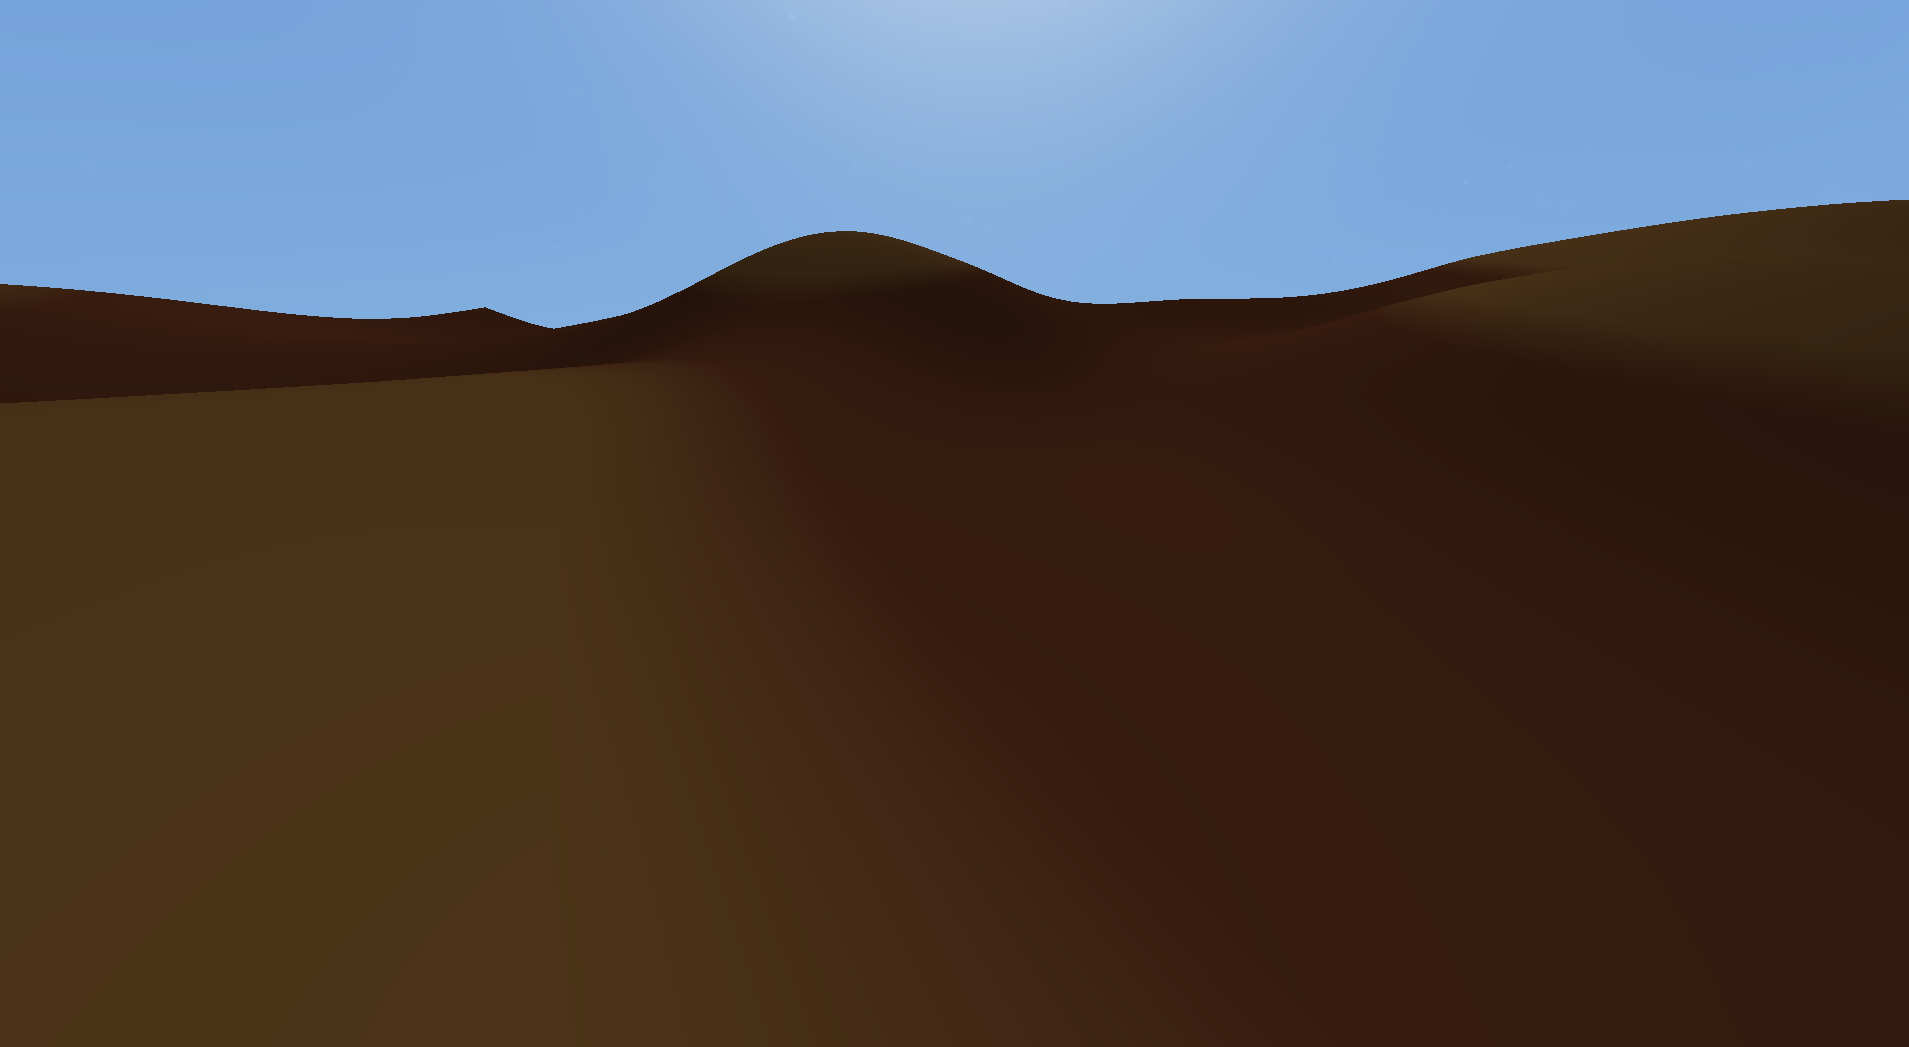
\includegraphics[width=0.8\textwidth]{chapters/implementation/sections/terrain/resources/octaves-1.png}
        \caption{Small number of octaves (1).}
    \end{subfigure}
    \hfill
    \begin{subfigure}{0.45\textwidth}
        \centering
        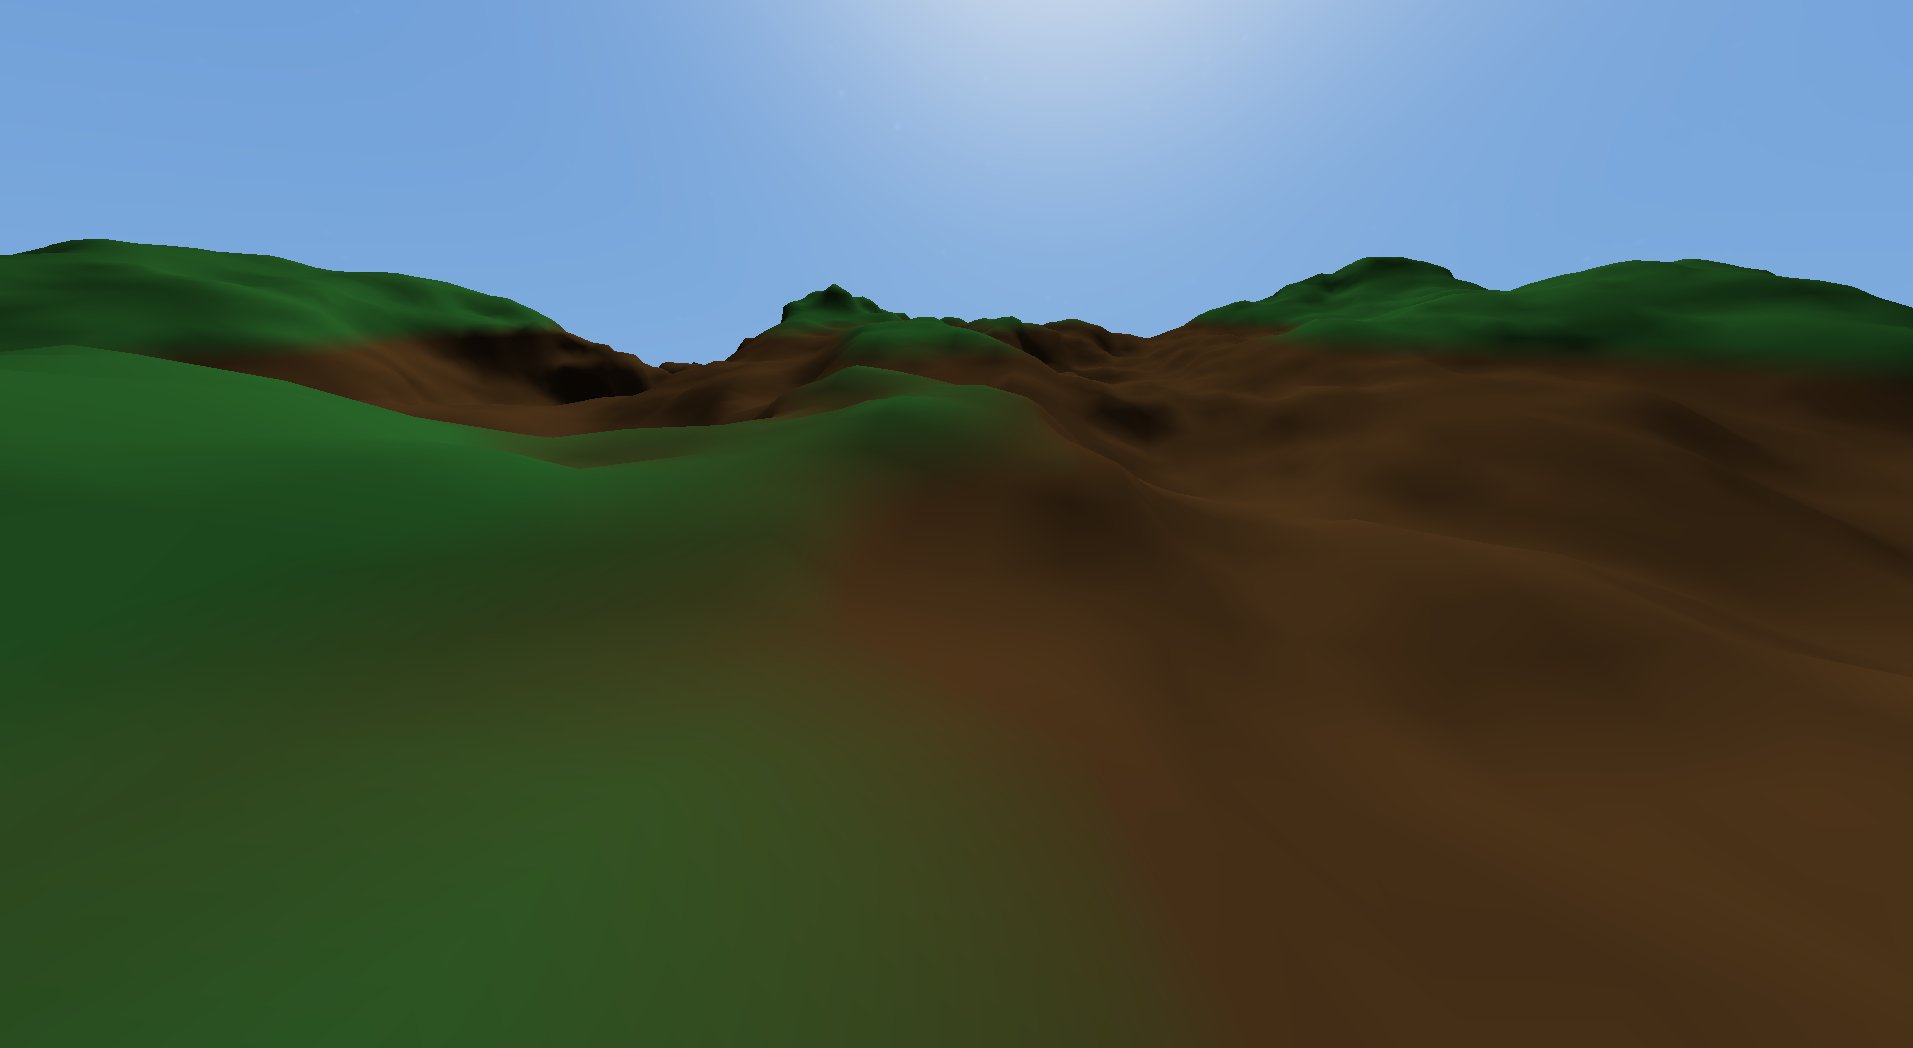
\includegraphics[width=0.8\textwidth]{chapters/implementation/sections/terrain/resources/octaves-5.png}
        \caption{Large number of octaves (5).}
    \end{subfigure}

    \centering
    \begin{subfigure}{0.45\textwidth}
        \centering
        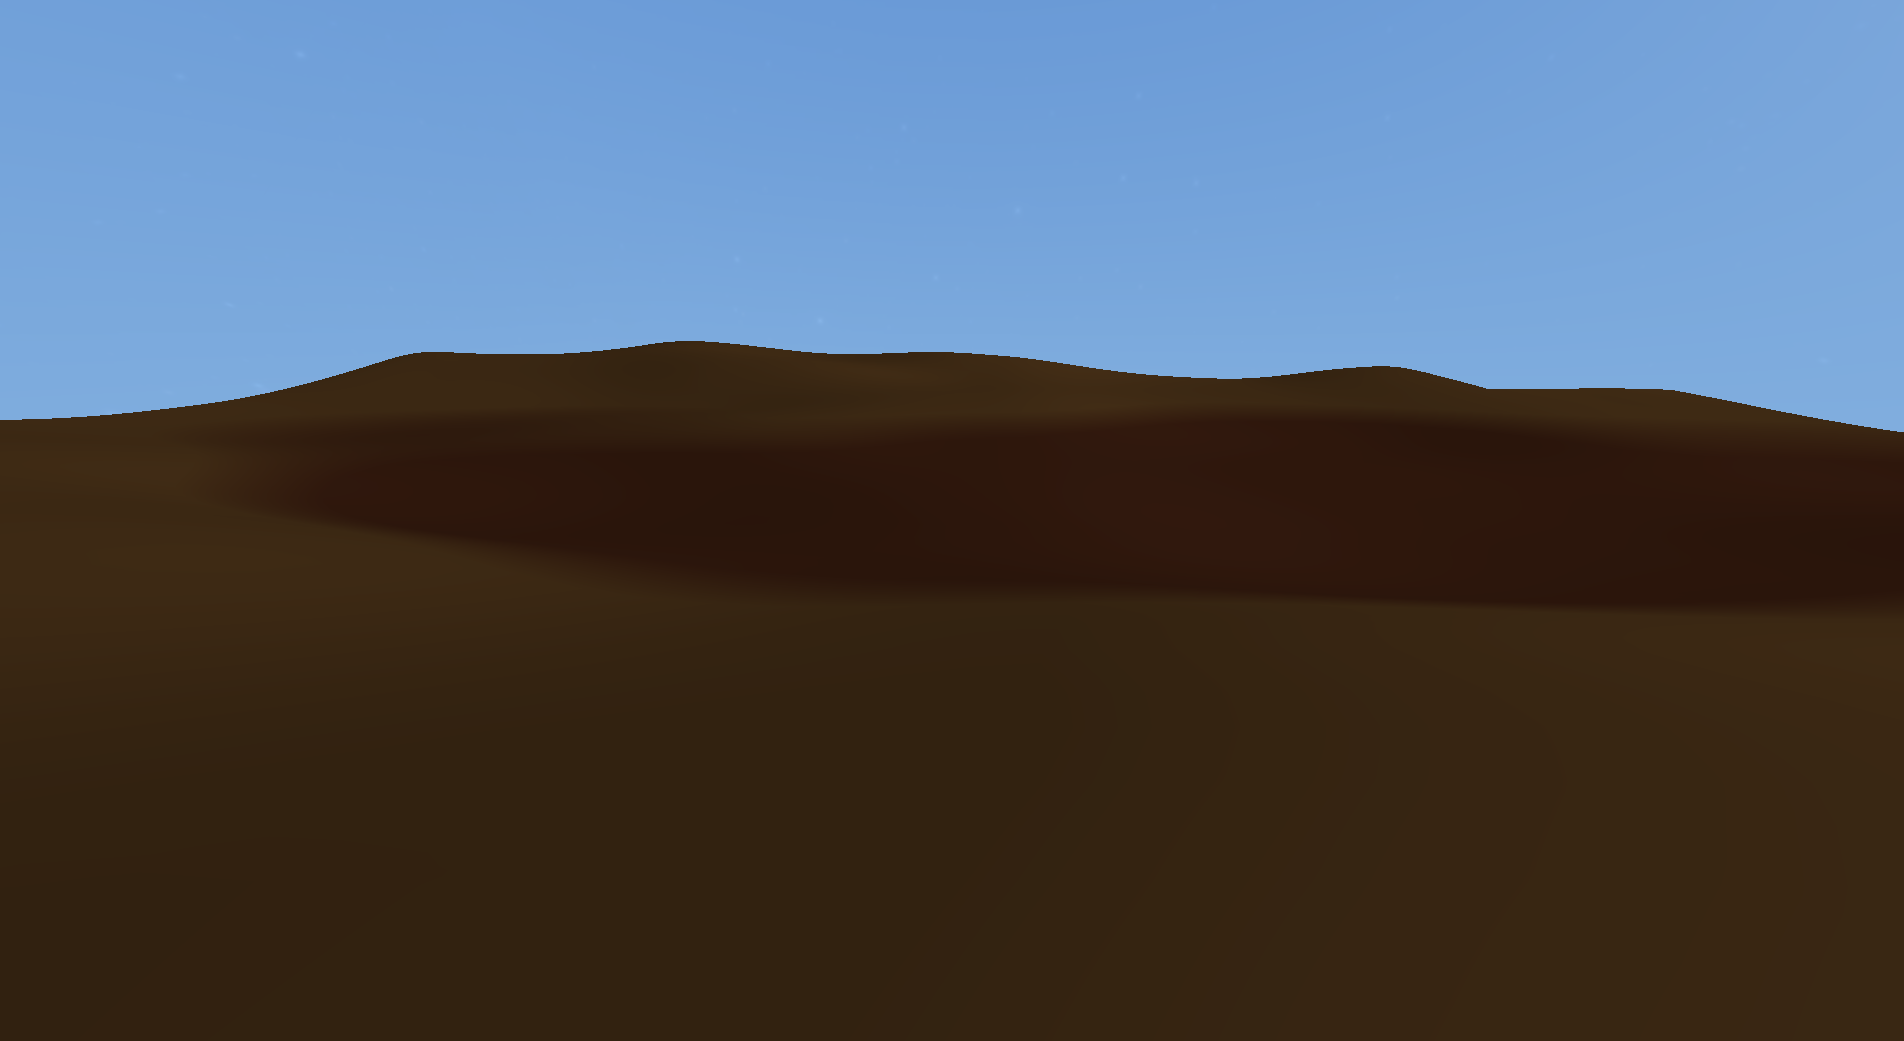
\includegraphics[width=0.8\textwidth]{chapters/implementation/sections/terrain/resources/initial-freq-0.1.png}
        \caption{Small initial frequency (1).}
    \end{subfigure}
    \hfill
    \begin{subfigure}{0.45\textwidth}
        \centering
        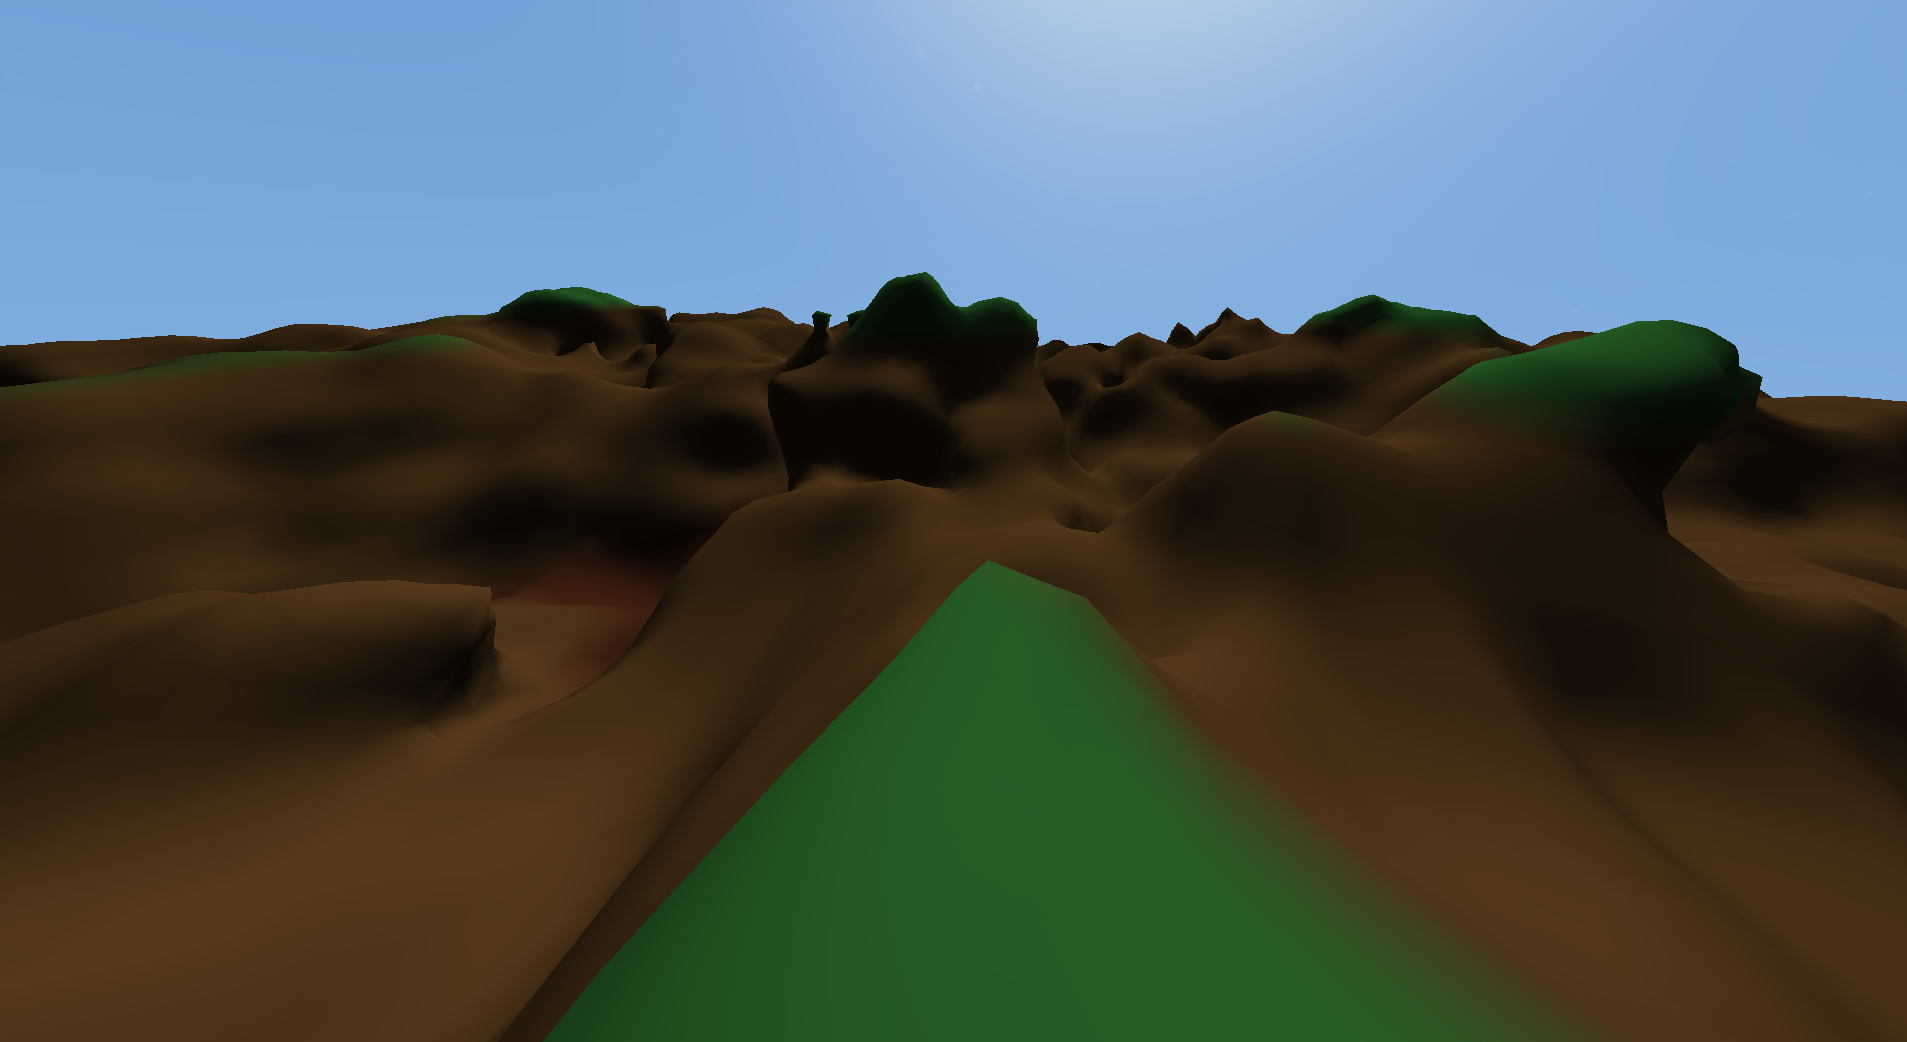
\includegraphics[width=0.8\textwidth]{chapters/implementation/sections/terrain/resources/initial-freq-0.5.png}
        \caption{Big initial frequency (0.5).}
    \end{subfigure}

    \centering
    \begin{subfigure}{0.45\textwidth}
        \centering
        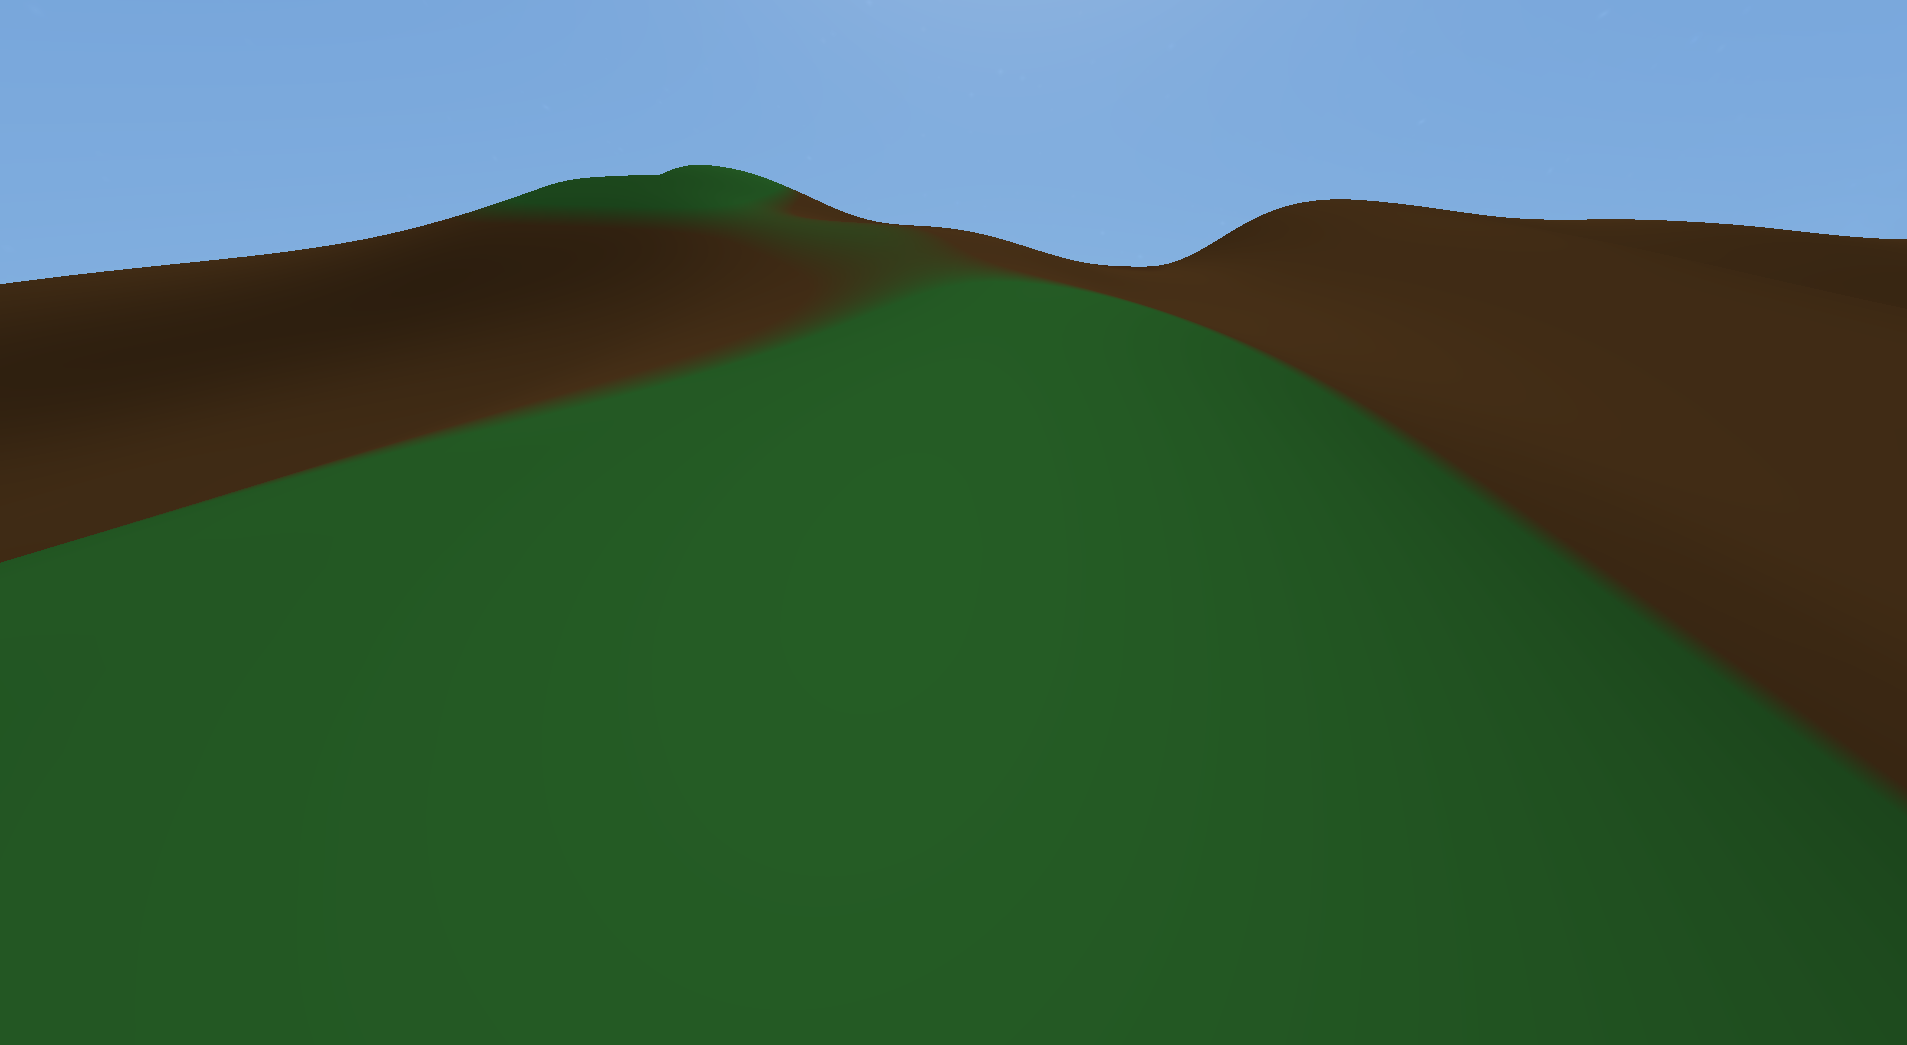
\includegraphics[width=0.8\textwidth]{chapters/implementation/sections/terrain/resources/freq-mul-0.5.png}
        \caption{Small frequency multiplier (0.5).}
    \end{subfigure}
    \hfill
    \begin{subfigure}{0.45\textwidth}
        \centering
        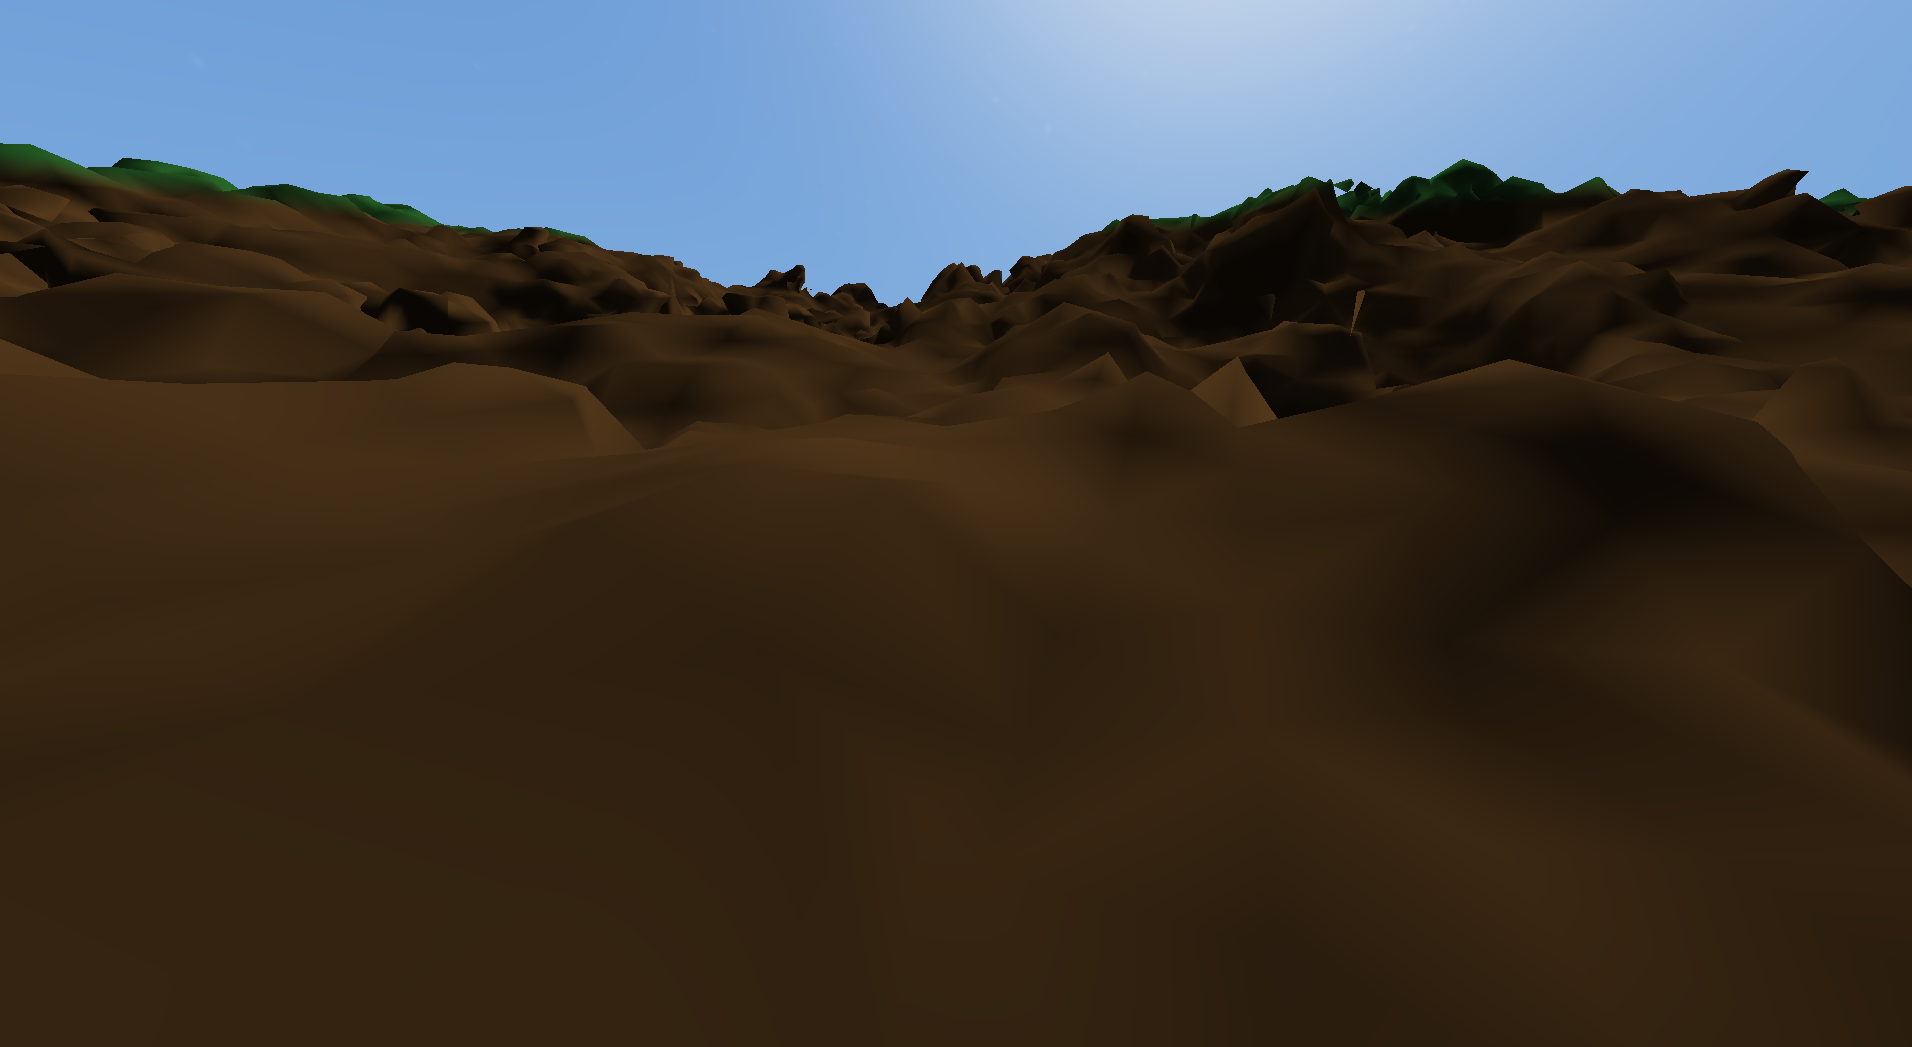
\includegraphics[width=0.8\textwidth]{chapters/implementation/sections/terrain/resources/freq-mul-5.png}
        \caption{Big frequency multiplier (5).}
    \end{subfigure}

    \centering
    \begin{subfigure}{0.45\textwidth}
        \centering
        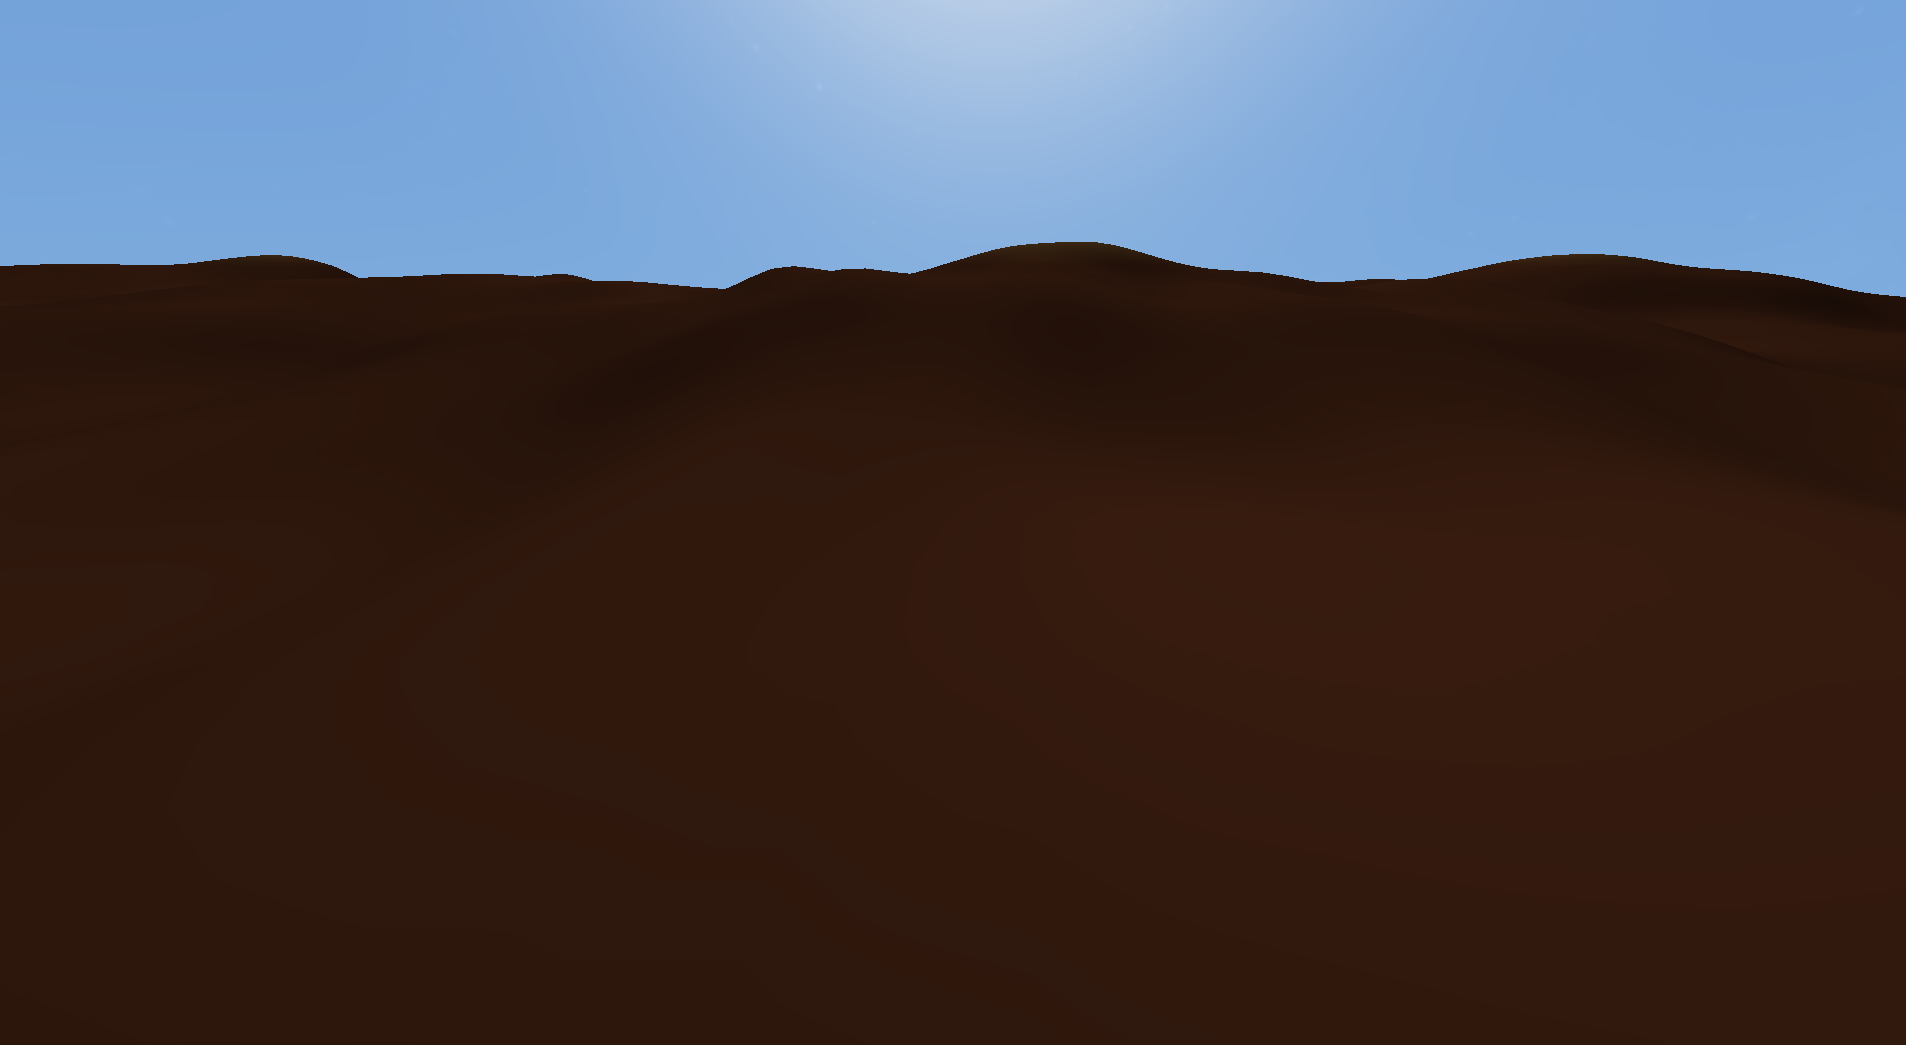
\includegraphics[width=0.8\textwidth]{chapters/implementation/sections/terrain/resources/initial-amp-8.png}
        \caption{Small initial amplitude (8).}
    \end{subfigure}
    \hfill
    \begin{subfigure}{0.45\textwidth}
        \centering
        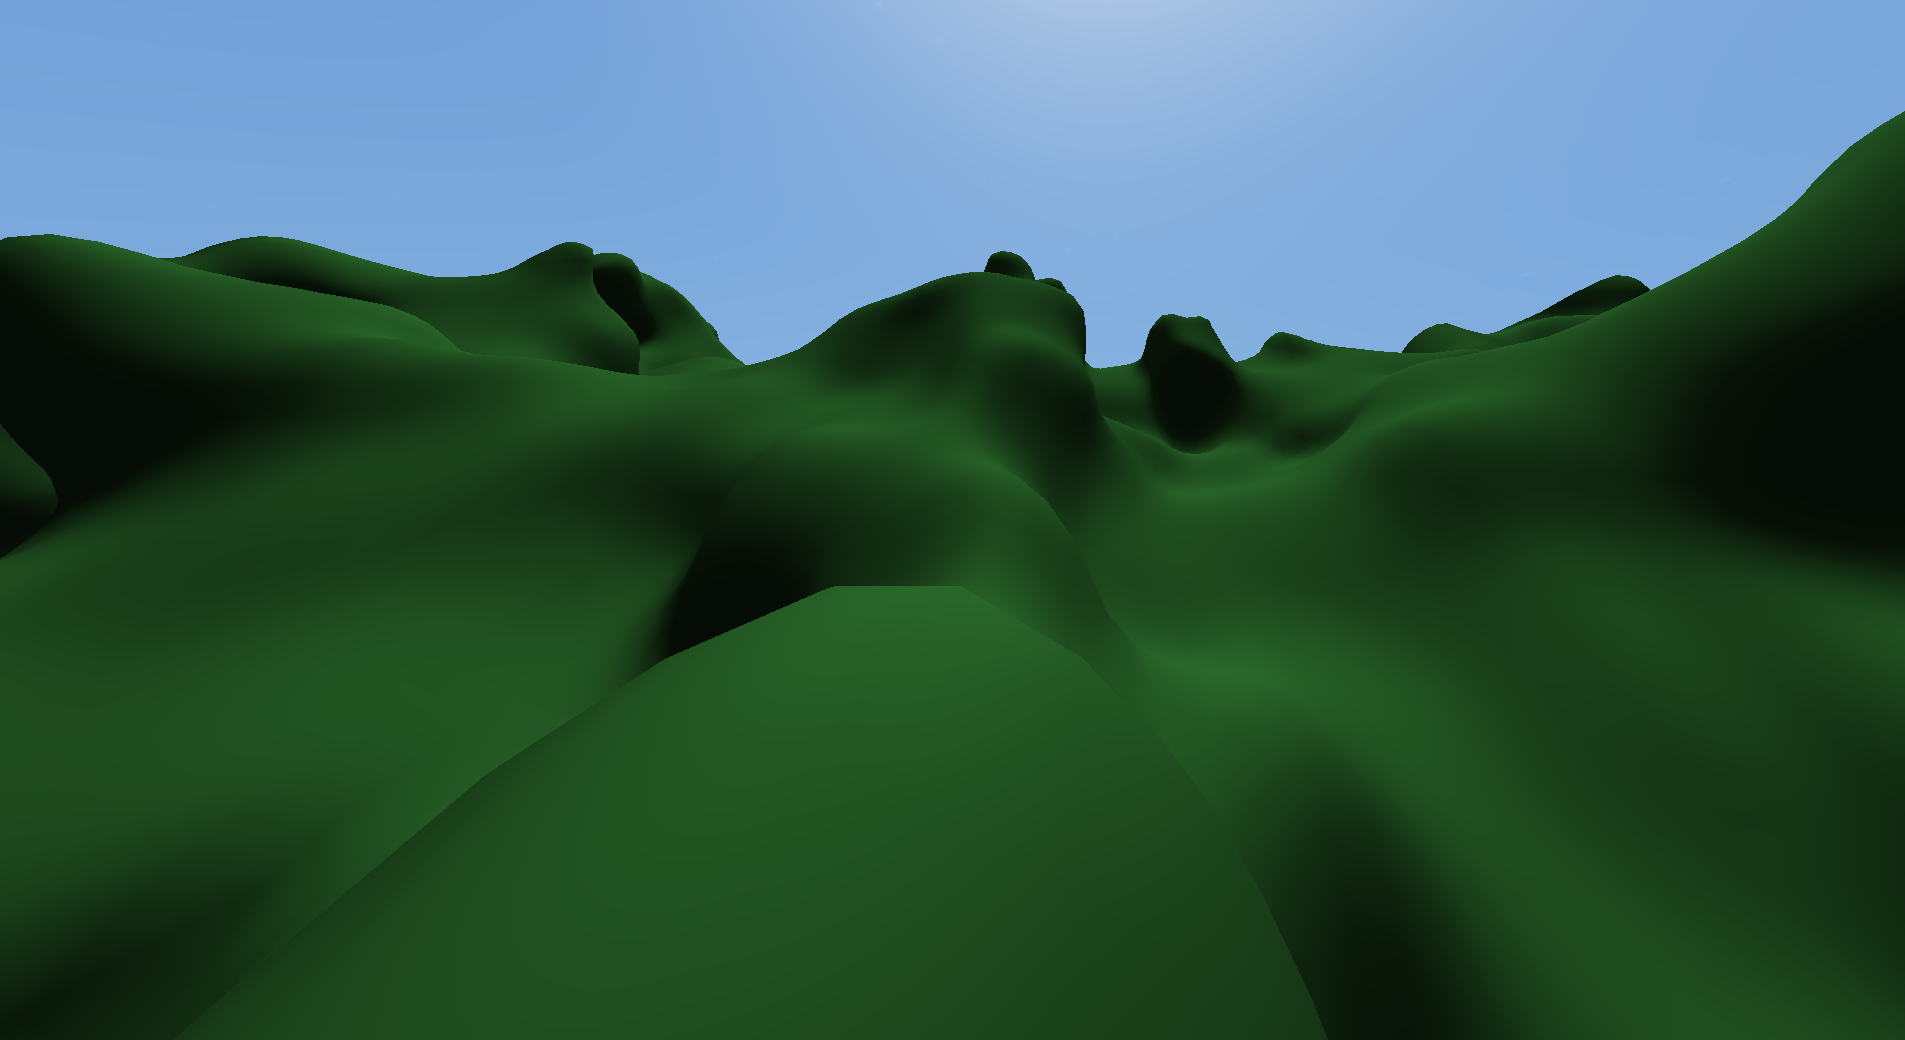
\includegraphics[width=0.8\textwidth]{chapters/implementation/sections/terrain/resources/initial-amp-32.png}
        \caption{Big initial amplitude (32).}
    \end{subfigure}

    \centering
    \begin{subfigure}{0.45\textwidth}
        \centering
        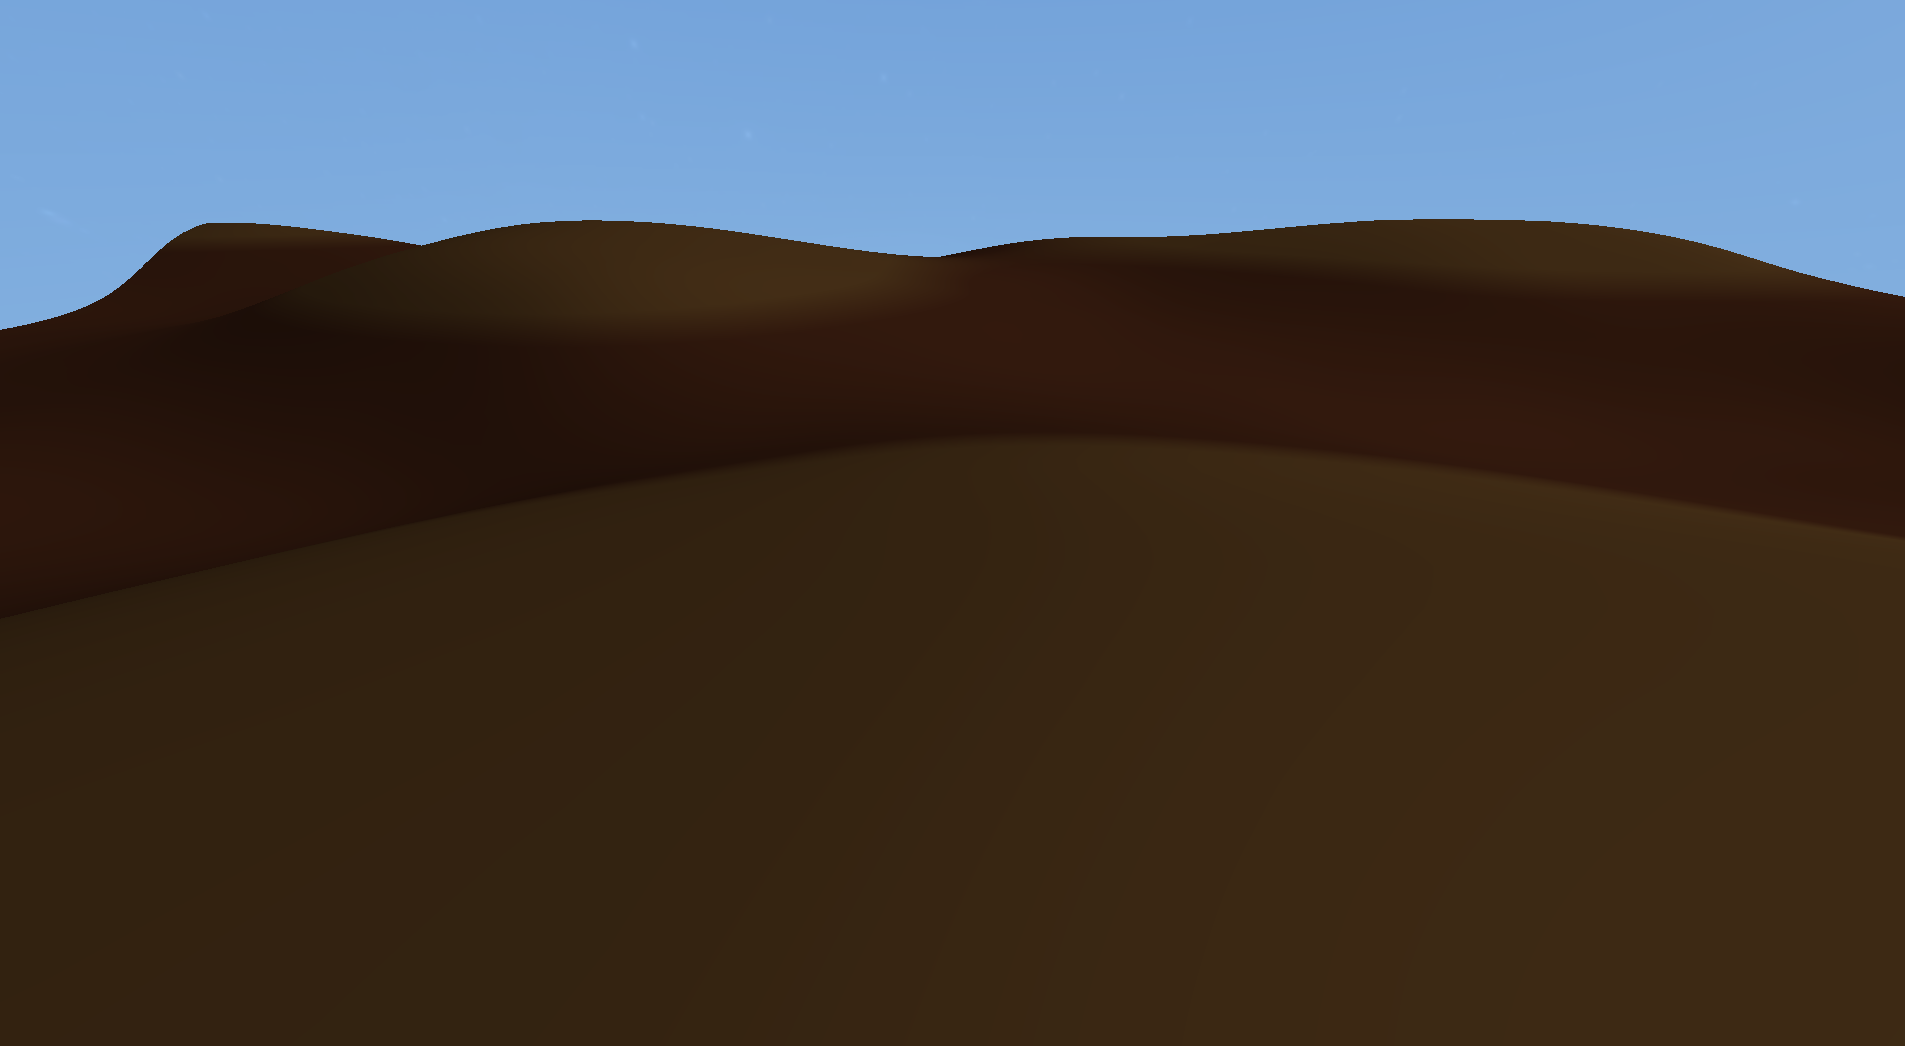
\includegraphics[width=0.8\textwidth]{chapters/implementation/sections/terrain/resources/amp-mul-0.1.png}
        \caption{Small amplitude multiplier (0.1).}
    \end{subfigure}
    \hfill
    \begin{subfigure}{0.45\textwidth}
        \centering
        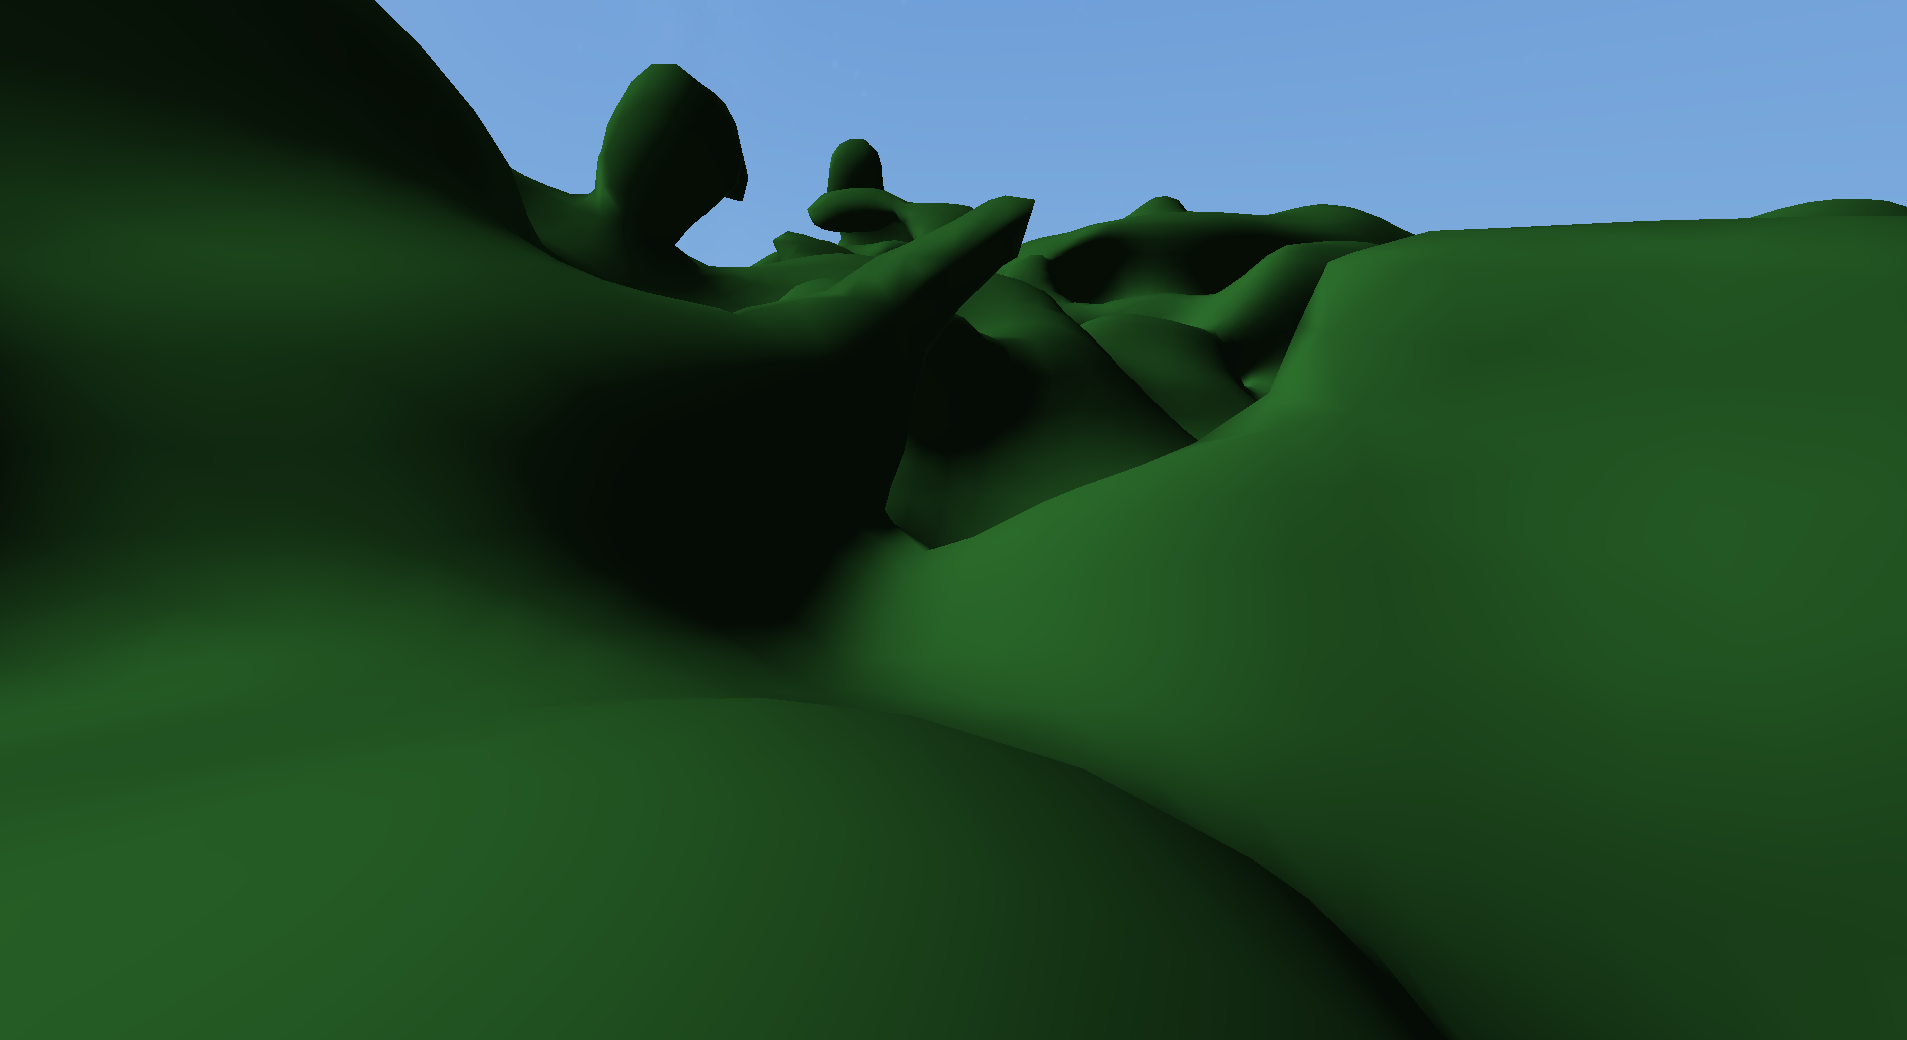
\includegraphics[width=0.8\textwidth]{chapters/implementation/sections/terrain/resources/amp-mul-1.png}
        \caption{Big amplitude multiplier (1).}
    \end{subfigure}

    \caption{Scalar field parameter comparison.}
    \label{fig:argument_comparison}
\end{figure}
\subsection{Chunks}
As mentioned before one of the most important things for the terrain was a way to edit it.
Editing the whole terrain at once would be very slow and not very efficient.
Thus the terrain is split into chunks -- cubically shaped, distinct sections of the world.
Each chunk is a separate object and can be edited independently.
This solution is much more efficient but it also causes some problems.

One problem is that the terrain is not continuous.
Every time we edit a chunk we need to make sure that the edges of the chunk are behaving in the same way as the edges of the neighboring chunks.
This is done by making sure that when a function that updates one chunk is called it is also called with the same parameters for other affected chunks.
Without this, the terrain would have holes in it between chunks which is shown in a screenshot from an early version of the game in \autoref{fig:gaps_between_chunks}.

Another problem is that the algorithm we used for generating the terrain, described in \autoref{subsec:marching_cubes}, calculates normal vectors based on the values of the scalar field around the point at which the normal is calculated.
This means that the normal vectors at the edges of the chunks have to be calculated differently.
This is a common problem with the algorithm and it is visualized in \autoref{fig:problem_with_normals_at_chunk_edge}.
The most common solution and the one we used is extending the scalar field by one layer of points around the chunk.
This means that the chunk contains information about the scalar field outside of the chunk itself.
That way the normal vectors can be calculated the same way for all points in the chunk.

\begin{figure}[!htb]
    \centering
    \begin{minipage}{0.45\textwidth}
        \centering
        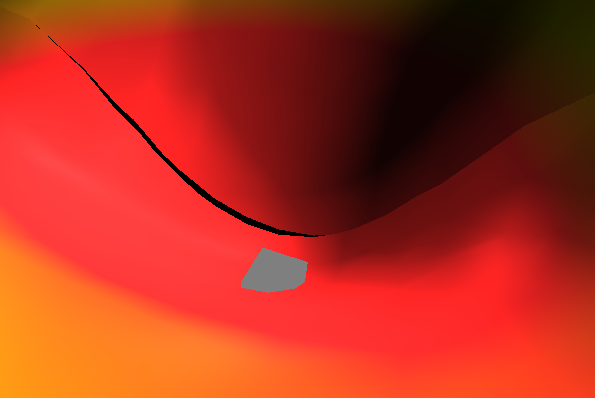
\includegraphics[width=0.8\textwidth]{chapters/implementation/sections/terrain/resources/chunk_edges_gaps.png}
        \caption{Gaps between chunks.}
        \label{fig:gaps_between_chunks}
    \end{minipage}\hfill
    \begin{minipage}{0.45\textwidth}
        \centering
        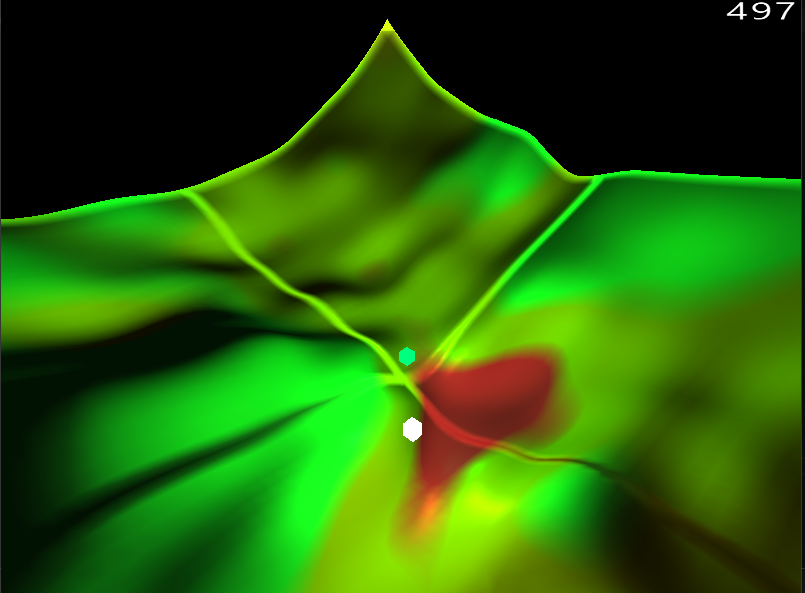
\includegraphics[width=0.8\textwidth]{chapters/implementation/sections/terrain/resources/chunk_edges_normals_problem.png}
        \caption{Problem with normals at chunk edges.}
        \label{fig:problem_with_normals_at_chunk_edge}
    \end{minipage}
\end{figure}

There are potentially infinitely many chunks in the world, which is why chunks are only loaded/created when a player is close to them.
They are also unloaded when the player moves far enough away from them.
When that happens they are saved to disk and removed from RAM.
The same thing happens when the game is closed.
\subsection{Marching Cubes} \label{subsec:marching_cubes}
The idea of the algorithm is described in \autoref{sec:theory_theory_marching_cubes}.
This section will describe the way the algorithm was implemented in our project.

To make the mesh look smoother we interpolate the position of the vertices along the edges based on the values of the scalar field at the cube's vertices.
This is done by using the linear interpolation given by equation \autoref{eq:linear_interpolation}.
\begin{equation}
  \label{eq:linear_interpolation}
  P = V_1 + \frac{\text{IsoLevel} - v_1}{v_2 - v_1} (V_2 - V_1)
\end{equation}
where $P$ is the resulting position of the vertex, $V_1$ and $V_2$ are the positions of the vertices of the cube, $v_1$ and $v_2$ are the values of the scalar field at the vertices and IsoLevel is the isolevel of the mesh.

This gives us a mesh.
To make the impression of a light reflecting off a smooth surface we also need to calculate the normal vectors for each vertex.
The normal vectors in each point of the scalar field are calculated using \autoref{eq:normal_vector}
\begin{equation}
  \label{eq:normal_vector}
  n(x, y, z) = \begin{bmatrix}
    s(x + 1, y, z) - s(x - 1, y, z) \\
    s(x, y + 1, z) - s(x, y - 1, z) \\
    s(x, y, z + 1) - s(x, y, z - 1)
  \end{bmatrix}
\end{equation}
where $s(x, y, z)$ is the value scalar field function at $(x,y,z)$ and $n(x, y, z)$ is the normal vector at that point.
These vectors are used to calculate the mesh normals using the same interpolation used for the mesh \autoref{eq:linear_interpolation}.

The last part of creating the mesh is assigning colors to each vertex.
Each point of the scalar field is assigned a type which is described in \autoref{subsec:scalar_field} and each type has a corresponding color.
The color of each vertex of the mesh is calculated by interpolating the colors of the points of the scalar field using \autoref{eq:linear_interpolation}.
\subsection{Editing terrain} \label{sec:terrain_editing}
Editing terrain is done by changing the values of the scalar field.
When a chunk is first created the values of the scalar field are calculated for each point in the chunk and then saved.
This allows for the scalar field values to be edited.
When a chunk is edited the values of the scalar field are recalculated for the edited points and the points around them.
The player can choose a point to build or mine at.
Values of the scalar field close to that point are then changed based on the pickaxe the player uses and how long they mine for.
The closer the point to the chosen point $c$ the more it is affected.
We propose to use a 3D Gaussian function to calculate exactly how much each point is affected to make the terrain look smooth after the modification.
The function is shown in \autoref{eq:gaussian}.

\begin{equation}
    \label{eq:gaussian}
    f(x, y, z) = e^{-a \left((x - c_x)^2 + (y - c_y)^2 + (z - c_z)^2\right)}
\end{equation}

In \autoref{eq:gaussian} $x$, $y$ and $z$ are the coordinates of a point being edited, $c_x$, $c_y$ and $c_z$ are the coordinates of the chosen point (center of the modification) and $a$ is a constant.
Moreover, if the distance between the chosen point and the point being edited is greater than the range of the pickaxe, the point is not affected.

Once the values of the scalar field are updated the chunk is regenerated.
This is a very time-consuming process which is why it was moved to a second thread.
The communication between that thread and the main one is described in \autoref{sec:chunk-worker}.

\section{Chunk management system}\label{sec:chunk-worker}
The majority of the game logic is handled by a single thread.
The only two exceptions are the physics engine (external library) and the chunk management system.
The chunk management system is split between two threads: the main thread (the thread that the rest of the application is running on) and the \textit{chunk worker's} thread.
The worker's thread is concerned with operations that are either CPU-intensive or could take a long time to execute.
More specifically, the chunk worker is performing the following operations:
\begin{enumerate}
    \item loading saved chunks from disk and generating new chunks,
    \item saving chunks to disk,
    \item updating chunks.
\end{enumerate}
The system is built around the producer-consumer pattern, i.e. the main thread communicates with the worker's thread (and \textit{vice versa}) using queues.
It's important to note that depending on the stage of an operation either thread can be the \textit{producer} or the \textit{consumer}.
We will now describe the workflow for each of the operations mentioned before.

\subsection{Loading and generating chunks} \label{subsec:loading-and-generating}
On each render frame, the main thread calls the \texttt{UpdateCurrentPosition} method.
This method, based on the camera's current position and the render distance, determines which chunks should be loaded into the game.
If a chunk isn't already loaded or isn't queued for loading, the position of the chunk is enqueued into the \texttt{chunksToLoad} queue.

The worker thread in the \texttt{LoadChunks} function dequeues the positions of the chunks to be loaded from the disk.
If a chunk is not saved on the disk, it is generated.
The loaded/generated chunk is then enqueued into the \texttt{loaded} queue.

The main thread through the \texttt{ResolveLoaded} function dequeues a chunk and performs the following actions:
\begin{enumerate}
    \item creates a vertex array object for the chunk's mesh,
    \item creates a collision surface for the chunk,
    \item adds the chunk to the list of scene's chunks for rendering.
\end{enumerate}

It's worth noting that the operations in \texttt{ResolveLoaded} function have to be performed on the main thread because they interact with OpenGL and the physics engine APIs.
\subsection{Saving chunks}
Saving chunks is handled by a process similar to the one discussed in \autoref{subsec:loading-and-generating}.
On each frame, the main thread in the \texttt{DeleteChunks} function determines which chunks are too far from the player and thus should be removed from the game and saved to disk.
Positions of these chunks are enqueued into the \texttt{chunksToSave} queue, and their resources are freed.
More precisely, the removal takes place only if the number of chunks in the game exceeds a certain limit.
This is so that chunks are not deleted and loaded again constantly when the player moves back and forth between chunks.

The worker thread dequeues chunks' positions from the \texttt{chunksToSave} queue and saves the scalar field associated with a given chunk on the disk.
\subsection{Updating chunks}
Terrain modification consists of two main steps:
\begin{enumerate}
    \item the scalar field for the modified chunk has to be altered, which involves iterating over a 3-dimensional array of numbers and modifying the values stored in that array using some function,
    \item a new mesh has to be generated based on the new values of the scalar field.
\end{enumerate}
Since the modifications happen 60 times a second and the number of operations they require is rather big (of the order of the chunk size, i.e. $16^3$) it's unfeasible to do them on the main thread without severe lags.
Thus most of the work related to terrain modification is delegated to the worker thread.

The workflow for terrain modification can be described as follows.
The main thread in the \texttt{Pickaxe.ModifyTerrain} method determines which chunks are going to be affected by the terrain modification, and adds them to a buffer \texttt{buffer}.
Once all the chunks are in \texttt{buffer}, we set the \texttt{IsProcessingBatch} flag to \texttt{true} (while set to true, no further terrain modifications will be registered) and enqueue each of them into the \texttt{modificationsToPerform} queue along with some additional information (passed in the form of an instance of \texttt{ModificationArgs} struct) necessary to perform the modification.
A very important piece of information is the \texttt{batchSize} which is the size of \texttt{buffer} (its importance will become apparent later).

The worker thread dequeues chunks from the \texttt{modificationsToPerform} queue.
It modifies the scalar field using the information passed in \texttt{ModificationArgs} and generates a new mesh based on the scalar field.
Once new vertices for the mesh are calculated, it enqueues the chunk together with \texttt{batchSize} (retrieved from \texttt{modificationArgs}) into the \texttt{updatedChunks} queue.

In the \texttt{ResolveUpdated} function the main thread dequeues the \texttt{(chunk, batchSize)} pair from the \texttt{updatedChunks} queue and adds \texttt{chunk} to the \texttt{currentBatch} list.
Once the number of chunks in \texttt{currentBatch} is equal to \texttt{batchSize} of the dequeued chunk, it means that the main thread has "received back" all of the chunks from a single modification call.
The main thread then updates the GPU buffers with the new vertices of the chunk's mesh and updates the shape of the collision surface in the physics engine for each chunk from \texttt{currentBatch}.
Once the whole \texttt{currentBatch} is updated, the \texttt{IsProcessingBatch} flag is set back to false.

The whole process is depicted in \autoref{fig:chunk-worker}.
\begin{figure}[!htb] % https://drive.google.com/file/d/1TzJouYAys_fz1GkhppZsqoh9yFn62twL/view?usp=sharing
    \centering
    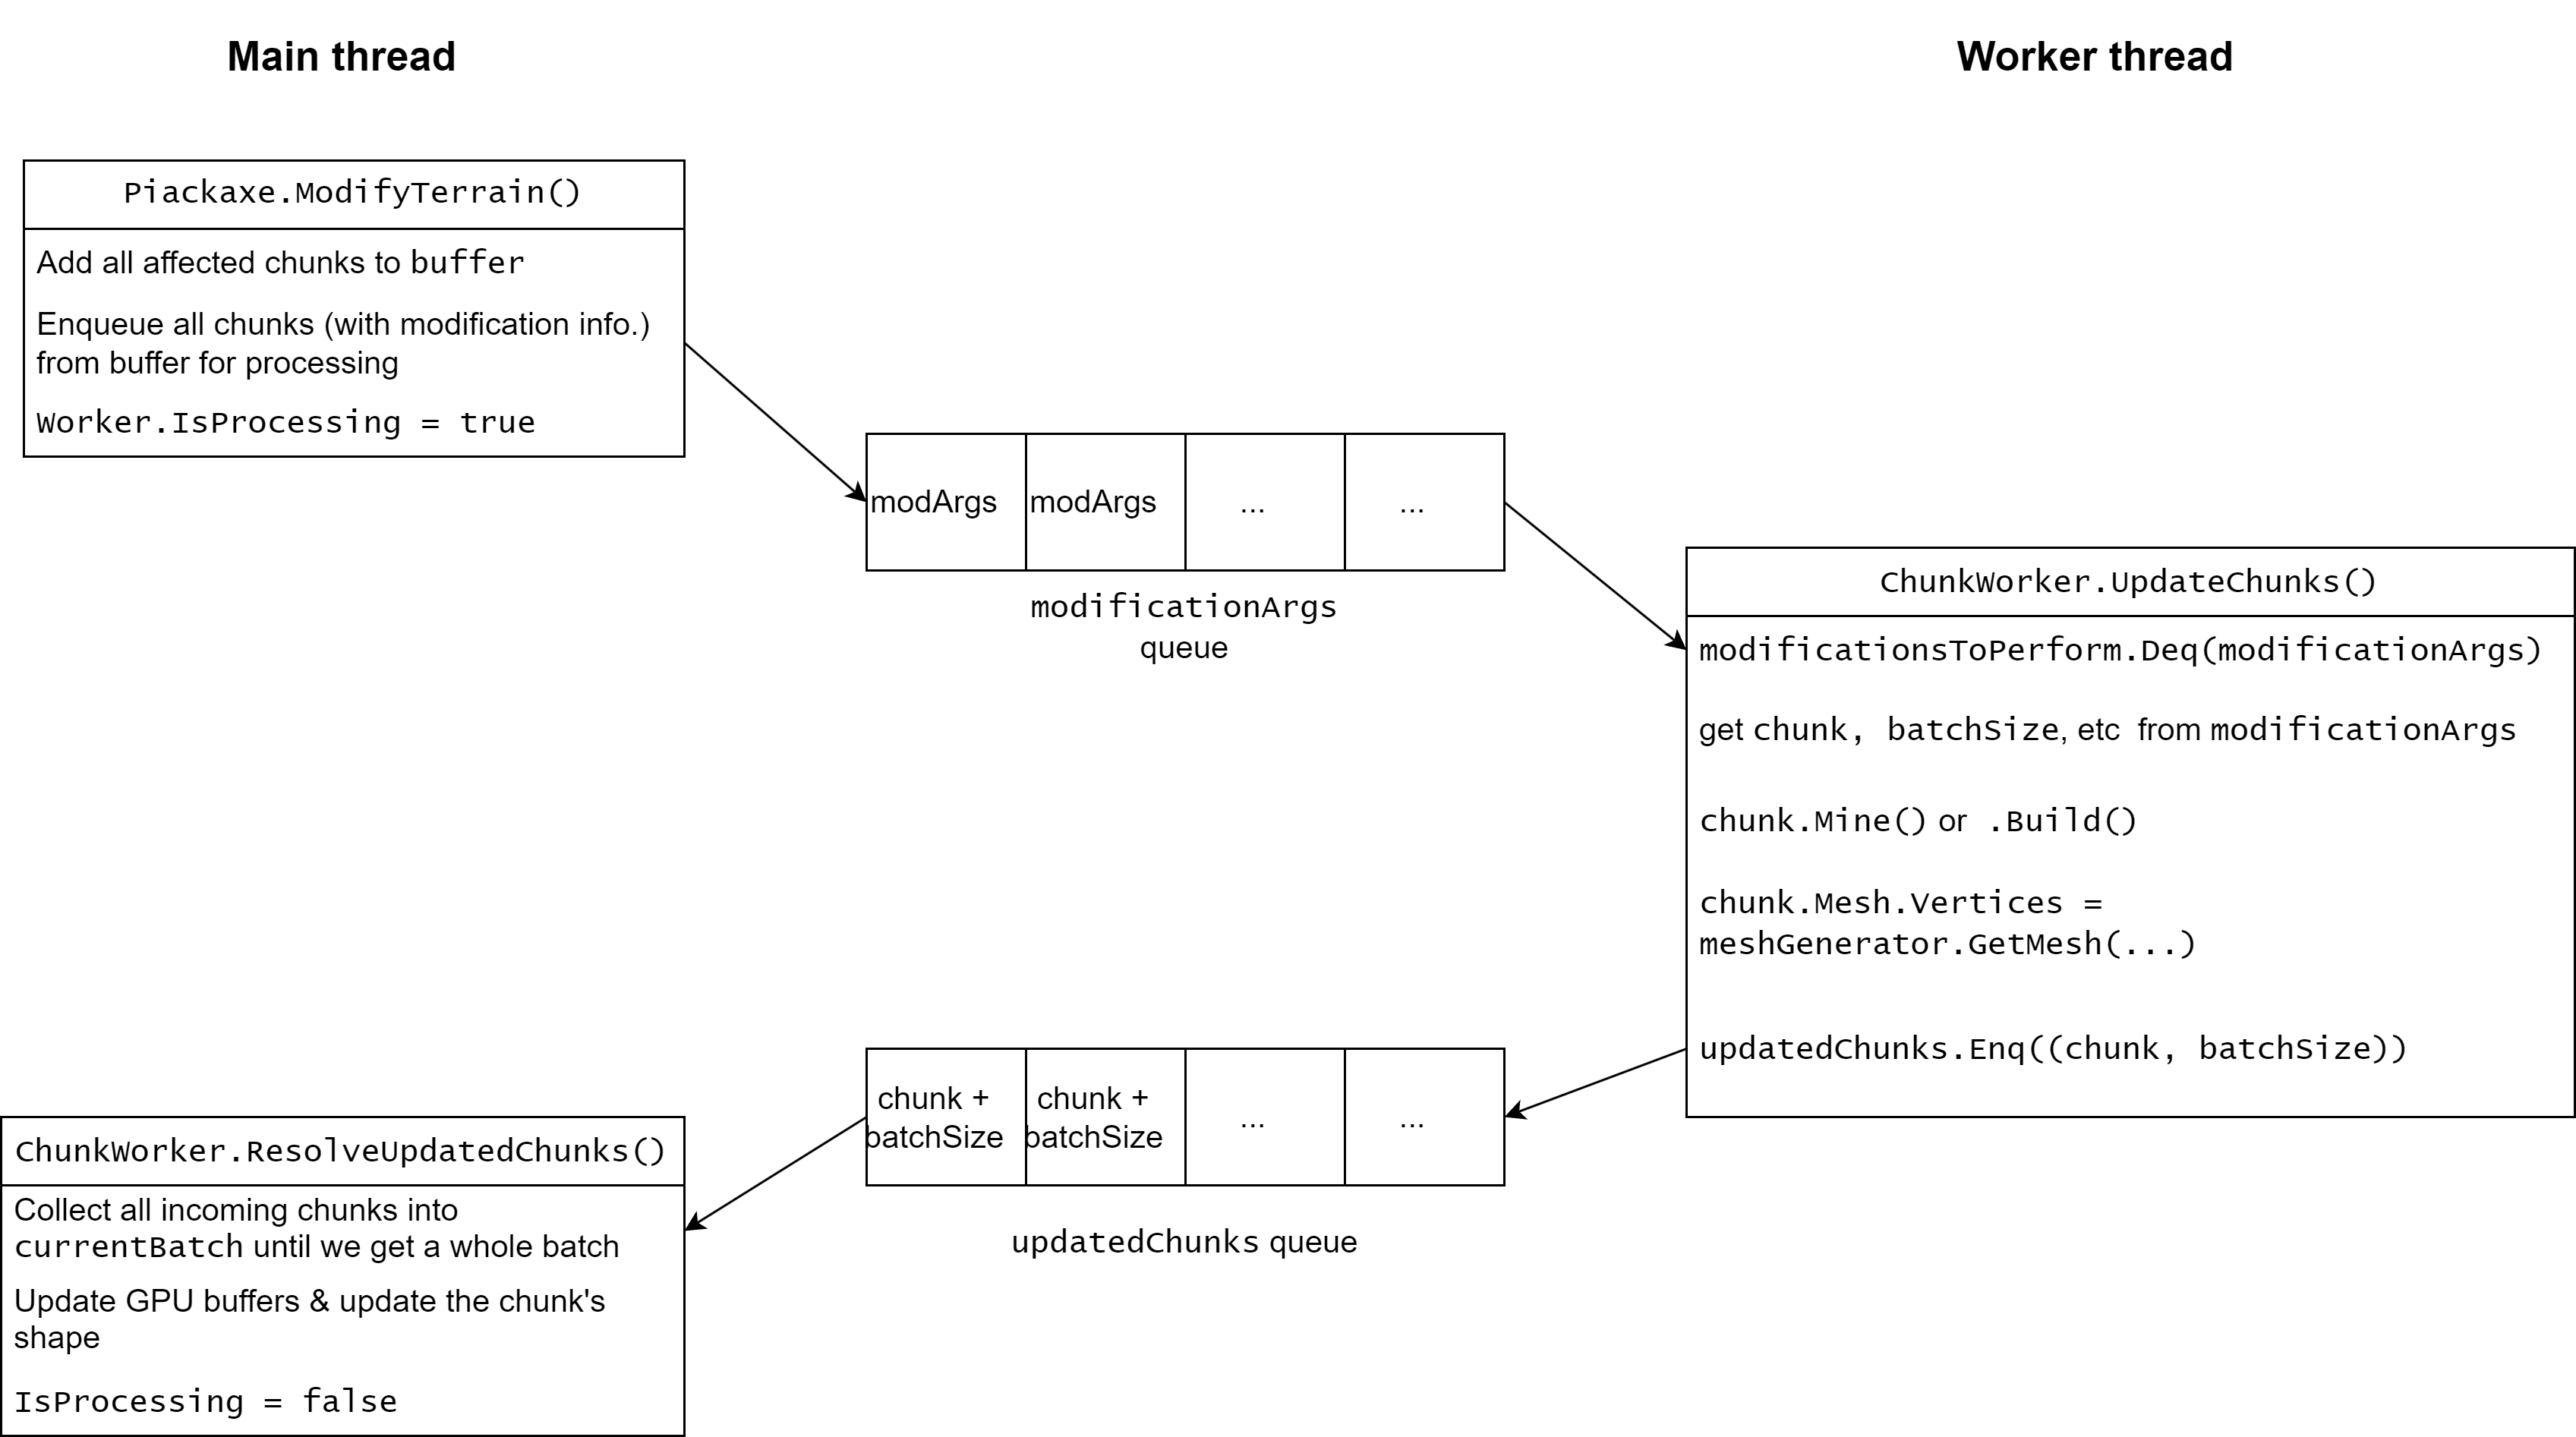
\includegraphics[width=1\textwidth]{chapters/implementation/sections/chunk_management_system/resources/chunkWorker.drawio.png}
    \caption{Terrain modification in the chunk management system}
    \label{fig:chunk-worker}
\end{figure}

The reason for processing chunks in batches rather than individually is simple.
If we modify chunks one by one it may be the case that when the terrain is rendered, one chunk has already been modified, while its neighbor has not, resulting in a visible gap between the two.
This problem can be seen in \autoref{fig:gaps-between-chunks-chunk-worker} which comes from an early stage of the game's development.
\begin{figure}[!htb]
    \centering
    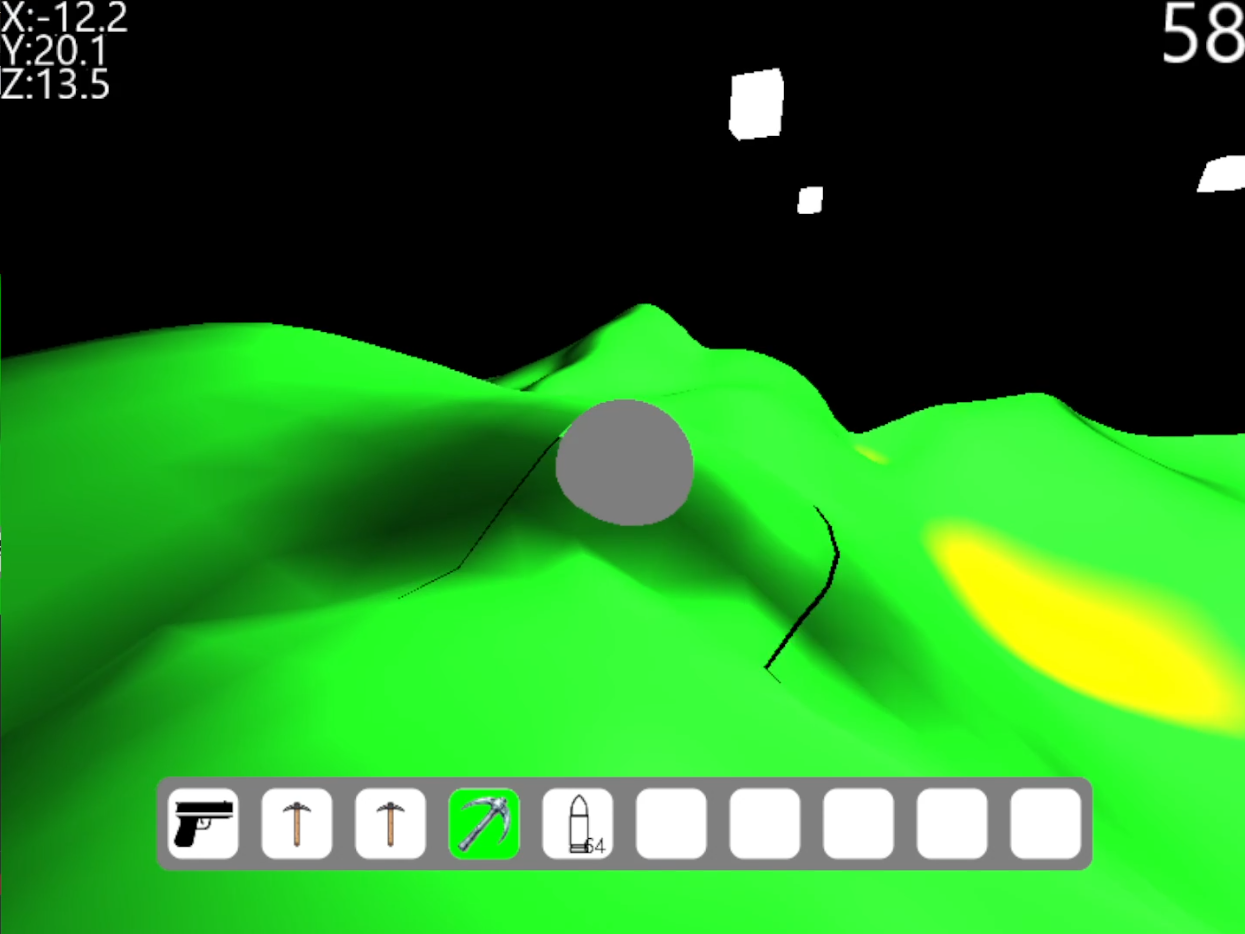
\includegraphics[width=0.6\textwidth]{chapters/implementation/sections/chunk_management_system/resources/gaps-between-chunks.png}
    \caption{Gaps between chunks appearing during terrain modification}
    \label{fig:gaps-between-chunks-chunk-worker}
\end{figure}

One drawback of this approach is that the main thread doesn't register new chunks for modification while the whole previously enqueued batch hasn't been processed.
This could cause the modification rate to be irregular should the main thread "drop" a lot of modifications.
To deal with this problem, the modification depends on the time elapsed between two modifications.
\section{Rendering}
Every game object exposes a \texttt{Render()} method.
The \texttt{Render} methods' signatures differ slightly across different game objects, but they usually take camera position, shader and space curvature as arguments.
At the time of writing, there are four shaders available for 3D rendering:
\begin{enumerate}
    \item light source shader,
    \item model shader,
    \item object shader,
    \item skybox shader.
\end{enumerate}
Model shader is used for rendering animated models, whereas light source and object shaders are used for rendering "static" bodies.
The light source shader is extremely basic: it doesn't take into account other light sources and colors the body uniformly.
The \texttt{Render} method typically interacts directly with the OpenGL interface, i.e. sets up the uniforms, binds VAOs and makes a draw call.
In the case of 2D rendering, \texttt{HudShader} class is used.
The skybox shader is used for rendering the \textit{skybox} i.e. a background used for the scene.

\section{User interface} \label{sec:two_dimensional_graphics}
OpenGL is a low-level graphics API.
It offers a set of functions to draw points, lines, and triangles.
It does not offer any functions to draw circles, ellipses, or other shapes.
That includes drawing text.
Because of that adding the heads-up display (HUD) and the Menu to the game is not as simple as we would like it to be.
In this chapter, we describe how we draw 2d elements in our application.

\subsection{Textures} \label{sec:textures}
OpenGL does offer a way to draw images.
To draw an image you have to create a texture.
This texture is then passed to a shader.
You also have to create a VAO which contains vertices for a rectangle.
Each vertex has a position and a texture coordinate.
These texture coordinates are used to sample the texture using built-in shader functions.

Each image we want to draw can be represented by a texture.
For each image we want to draw, we can create a texture and pass it to the shader.
While this approach works, it is not very efficient.
Passing textures to the shader is a slow operation.
Because of that, we want to use as few textures as possible.
We can do that by combining multiple images into one.
We create Sprite Sheets which contain multiple images.
Each image in a sprite sheet (sprite) has a position and a size.
We can use this information to calculate the texture coordinates for each sprite.
We pass this information to the shader and use it to sample the correct part of the texture.
This way, we can pass a single texture to the shader and draw multiple images with it.

In our application, we have 2 sprite sheets.
The first one contains the images for the HUD.
This includes the inventory and all the items in it.
This sprite sheet is stored as a PNG file.
Sprite sheet with the inventory can be seen in \autoref{fig:inventory}.
It also has a JSON file that contains the position and size of each sprite which can be seen in \autoref{lst:inventory_sprite_sheet_json}.
The second sprite sheet contains the images of all letters and symbols used in the game.
This one is not stored in a file.
Instead, it is generated at runtime right after the program launches.
It uses SkiaSharp library to create a bitmap with all the ASCII characters.
This bitmap is then converted to a texture, which we call the symbol texture.
The position and size of each symbol are calculated using the font metrics.

These techniques are used to draw the HUD and the Menu.
Both of those are described in this chapter.

\begin{figure}[h]
    \centering
    \begin{subfigure}{0.45\textwidth}
        \centering
        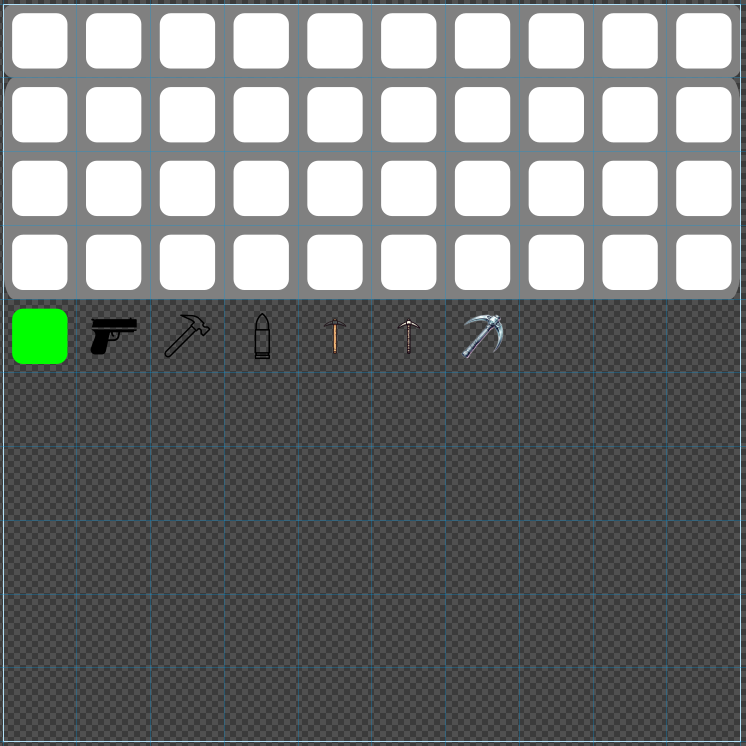
\includegraphics[width=0.8\textwidth]{chapters/implementation/sections/two_dimensional_graphics/resources/SpriteSheet.png}
        \caption{PNG file}
        \label{fig:inventory_texture}
    \end{subfigure}\hfill
    \begin{subfigure}{0.45\textwidth}
        \begin{lstlisting}[language=json,firstline=1]
    {
        "width": 10,
        "height": 10,
        "items": [
            {
            "name": "hotbar",
            "x": 0,
            "y": 0,
            "width": 10,
            "height": 1
            },
        ]
    }
    \end{lstlisting}

        \caption{JSON file}
        \label{lst:inventory_sprite_sheet_json}
    \end{subfigure}

    \caption{Inventory Sprite Sheet}
\end{figure}
\subsection{Heads Up Display} \label{sec:hud}
The HUD encapsulates all the 2D elements that are drawn on top of the 3D scene while the game is running.
This includes:
\begin{itemize}
    \item Crosshair
    \item FPS counter
    \item Player position
    \item Inventory
\end{itemize}

The Crosshair is a simple cross in the middle of the screen.
It is used to help the player aim.
It consists of two lines and does not use any textures.

The FPS counter is a simple text that shows the current frame rate.
It is drawn in the top right corner of the screen.
It uses the symbol's texture.

The player position is a simple text that shows the current position of the player.
It is drawn in the top left corner of the screen.
It uses the symbol's texture.

The inventory is a collection of images that represent the items the player has.
It is drawn at the bottom of the screen.
It uses both the item's texture containing the HUD items and the texture containing the alphabet.
The images of the items are drawn first and then the text is drawn on top of them.

All the elements of the HUD have their positions and sizes.
Each element is either placed in some position on the screen or is placed relative to some other element.
\subsection{Menu} \label{subsec:menu}
The menu is a lot more complicated than the HUD which is described in \autoref{sec:hud}.
Because of that, we decided to create a framework for creating menus.
This framework was heavily inspired by Flutter \cite{flutter}.
It uses the same concepts and terminology.
The overall idea is that everything is a widget.
A widget is a class that has a \texttt{Render} method as well as a \texttt{GetSize} method.
The \texttt{Render} method takes a context that includes information about the position and size on the screen that the widget can render to.
Some widgets also have children so the overall structure of the menu is a tree of widgets.

An example of a widget is shown in \autoref{fig:example_widget}.
This widget renders the main menu of the game.
The rendering logic of this widget can be seen in \autoref{fig:widget_logic}.
The idea is as follows.
The root widget calls the render method of its child which is the \texttt{Background} widget.
The \texttt{Background} widget renders the background color.
Then the \texttt{Background} widget calls the render method of its child which is the \texttt{Column} widget.
This widget renders its children in a column but to do that it first needs to know the size of each of its children.
Based on that information it will call a render method of each child with the appropriate context.
Each child asks its children for their size recursively until it reaches a leaf widget.
The process stops at the leaf and the render method is called on the children of the column widget.

This is a simplified version of the rendering logic as each widget has multiple options and rules that change how it or its children are rendered.
For example, the \texttt{Column} widget has a \texttt{alignment} property which changes how the children are aligned.
The \texttt{Button} widget in the \autoref{fig:widget_logic} itself is a tree of widgets.

This approach to rendering the menu is very flexible and allows for a lot of customization.
It improves on the method used to render the HUD described in \autoref{sec:hud}.
This approach is not common in game development.
Usually, menus are created by putting elements on the screen at specific positions.
In this part, we believe that our approach is better than the traditional one and improves on approaches used in for example Godot \cite{Godot-Menu}.

\begin{figure}[h]
  \centering
  \begin{subfigure}{0.45\textwidth}
    \centering
    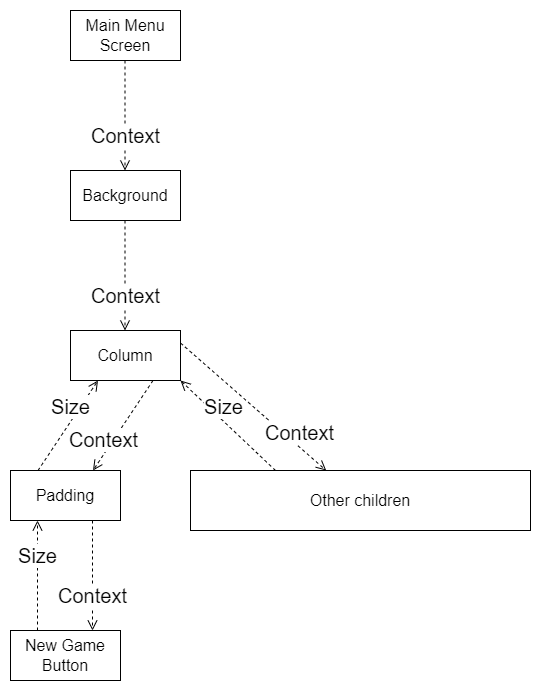
\includegraphics[width=0.8\textwidth]{chapters/implementation/sections/two_dimensional_graphics/resources/widget_logic.drawio.png}
    \caption{Widget rendering logic.}
    \label{fig:widget_logic}
  \end{subfigure}
  \hfill
  \begin{subfigure}{0.45\textwidth}
    \centering
    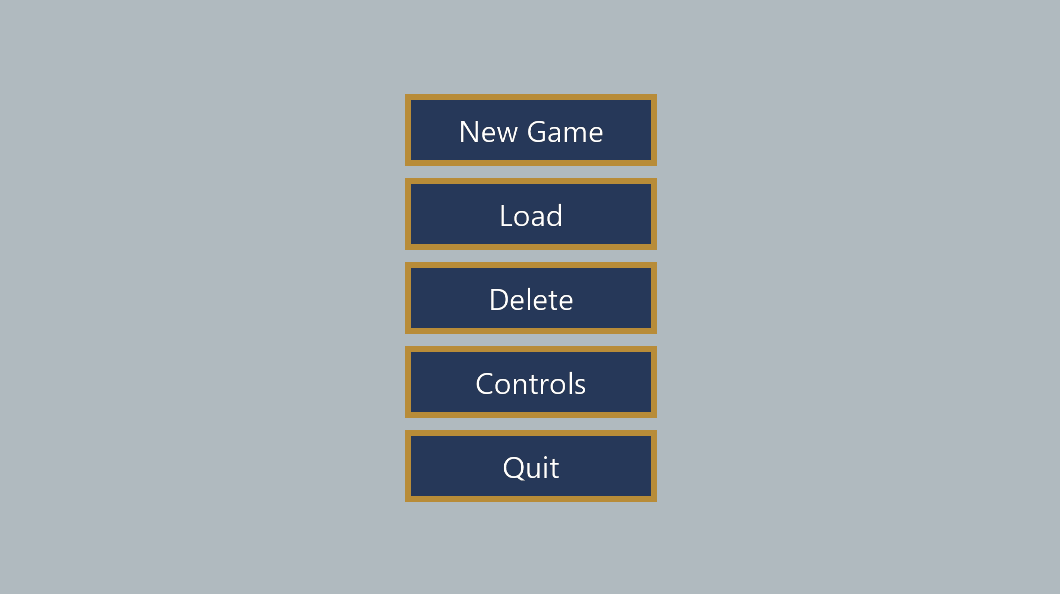
\includegraphics[width=0.8\textwidth]{chapters/implementation/sections/two_dimensional_graphics/resources/main-menu.png}
    \caption{Main menu.}
    \label{fig:example_widget}
  \end{subfigure}

  \caption{Example widget.}
\end{figure}
\todo{I removed the "Bots management" section. I think there wouldn't be much to write about that anyway.}